\documentclass[10pt,journal,compsoc]{IEEEtran}
\usepackage{balance}  % to better equalize the last page
\usepackage{graphics} % for EPS, load graphicx instead
\usepackage{times}    % comment if you want LaTeX's default font
\usepackage{url}      % llt: nicely formatted URLs

\usepackage{graphicx}
\usepackage{subfigure}
\usepackage{subfigure}
\usepackage{helvet}
\usepackage{courier}
\usepackage{diagbox}
\usepackage{amsmath}
\usepackage{multirow}
\usepackage{booktabs}
\usepackage{makecell}
\usepackage{amssymb}
\usepackage{threeparttable}
\usepackage[justification=centering]{caption}
\usepackage[linesnumbered,ruled,vlined,commentsnumbered]{algorithm2e}
\usepackage{color}
\usepackage{xcolor}
\usepackage[normalem]{ulem} % use normalem to protect \emph
\newcommand\hl{\bgroup\markoverwith
  {\textcolor{yellow}{\rule[-.5ex]{2pt}{2.5ex}}}\ULon}

%\ifCLASSOPTIONcompsoc
  % IEEE Computer Society needs nocompress option
  % requires cite.sty v4.0 or later (November 2003)
  %\usepackage[nocompress]{cite}
%\Else
%  % Normal Ieee
\usepackage{Cite}
%\Fi

\ifCLASSINFOpdf

\else

\fi

\hyphenation{op-tical net-works semi-conduc-tor}

\usepackage{hyperref}
\usepackage{breakurl}
%\newcommand\tabhead[1]{\small\textbf{#1}}
%\newtheorem{definition}{\bf Definition}
\newtheorem{definition}{Definition}
\def\boxend{\hspace*{\fill} $\Box$}
\newcommand{\comment}[1]{}
\renewcommand{\multirowsetup}{\centering}

\begin{document}

\title{Analyzing and Identifying Teens Stressful Periods and Stressor Events from a Microblog}

\author{Qi~Li,~Yuanyuan~Xue,~Liang~Zhao,~Jia~Jia~and~Ling~Feng~\IEEEmembership{Senior~Member,~IEEE}% <-this % stops a space
\IEEEcompsocitemizethanks{\IEEEcompsocthanksitem Dept. of Computer Science and Technology,
Centre for Computational Mental Healthcare Research, Institute of Data Science,
Tsinghua University, China.\protect\\
E-mail: \{liqi13,xue-yy12,jing-zhao11\}@mails.tsinghua.edu.cn, \{jjia,fengling\}@tsinghua.edu.cn
}}


%\thanks{Manuscript received April 19, 2005; revised September 17, 2014.}}

%\markboth{Journal of \LaTeX\ Class Files,~Vol.~13, No.~9, September~2014}%
%{Shell \MakeLowercase{\textit{et al.}}: Bare Demo of IEEEtran.cls for Computer Society Journals}

\IEEEtitleabstractindextext{%
\begin{abstract}
Increased health problems among adolescents caused by psychological stress have aroused worldwide attention.
Long-standing stress without targeted assistance and guidance
negatively impacts the healthy growth of adolescents, threatening the future development of our society.
So far, research focused on detecting adolescent psychological stress revealed from each individual post on microblogs.
However, beyond stressful moments, identifying teens stressful periods
and stressor events that trigger each stressful period
is more desirable to understand the stress from appearance to essence.
In this paper, we define the problem of identifying teens stressful periods and stressor events from the open social
media microblog.
Starting from a case study of adolescents' posting behaviors during stressful school events,
we build a poisson-based probability model for the
correlation between stressor events and stressful posting behaviors through a series
of posts on Tencent Weibo (referred to as the microblog throughout the paper).
With the model, we discover teen's maximal stressful periods and
further extract details of possible stressor events that cause the stressful periods.
We generalize and present the extracted stressor events
in a hierarchy based on common stress dimensions and event types.
Taking 122 scheduled stressful study-related events in a high school
as the ground truth, we test the approach on 124 students' posts from
January 1, 2012 to February 1, 2015,
and obtain some promising experimental results: (stressful periods: \emph{recall} 0.761, \emph{precision} 0.737, and $F_1$-\emph{measure} 0.734) and
(top-3 stressor events: \emph{recall} 0.763, \emph{precision} 0.756, and $F_1$-\emph{measure} 0.759).
The most prominent stressor events extracted
are in the \emph{self-cognition} domain, followed by the
\emph{school life} domain. This conforms to the adolescent psychological investigation result
that problems in school life usually accompanied with teens inner cognition problems.
Compared with the state-of-art top-1 personal life event detection approach, our stressor event detection method
is 13.72\% higher in \emph{precision}, 19.18\% higher in \emph{recall}, and 16.50\% higher in $F_1$-\emph{measure},
demonstrating the effectiveness of our proposed framework.
\end{abstract}

\begin{IEEEkeywords}
Adolescent, microblog, stressful period, stressor event.
\end{IEEEkeywords}}

\maketitle.

\IEEEdisplaynontitleabstractindextext

\IEEEpeerreviewmaketitle
\IEEEraisesectionheading{\section{Introduction}\label{sec:case study}}
\textbf{Motivation.}
Stress is an important health issue.
77\% of adults reported regularly experiencing physical symptoms caused by stress,
and an estimated 75\% to 90\% of visits to primary care physicians were stress-related~\cite{Hoffmann2015}.
Teens are more stressed out than adults.
According to an annual survey published by the American Psychological Association~\cite{Aleccia2014},
teens routinely said that their school-year stress levels were far higher than they thought
was healthy and their average reported stress exceeded that of adults.
Around 30\% of teens reported feeling sad or depressed because of stress and 31\%
felt overwhelmed. Another 36\% said that stress makes them tired and 23\% said they had
skipped meals because of it.
On average, teens reported their stress level was 5.8 on 10-point scale, compared with 5.1 for adults.
Stress seems to be getting worse for some teens, according to the survey.
About 31\% of kids said their stress level had increased in the past year,
twice as many as those who said it went down, and 34\% said they expected their stress level would rise in the coming year.
There is no doubt that with the fast speed of society and high expectation from adults and themselves,
teens will become more stressful than ever before.

Stress is the way human body responds to challenges.
The causes of stress are known as \emph{stressors} and there are literally hundreds of different types of stressors.
Any event that one finds threatening and difficult to cope with can be a potential cause of stress.
Typical stressor events
that may cause youth stress
include schoolwork and career decisions,
physical and cognitive changes of puberty, family and peer conflicts,
crammed schedules, dating and friendships, and so on.
The ways in which teens cope with these stressor events can
have significant short- and long-term consequences on their physical and
emotional health. Difficulties in handling stress can lead to mental health
problems, such as depression, anxiety disorders, and even suicide~\cite{Events2013}.
Due to the immaturity and lack of life experiences,
teenagers may not always take effective measures to deal with the stress.
Thus, timely discovery and effective intervention prevention of
adolescents�� mental disease is necessary and urgent.

\textbf{Existing solutions.}
Signs of teens stress could show up in their behaviors, emotions, and bodies, and can thus be
analyzed and discovered through various psychological signals
(e.g. heart rate variability HRV~\cite{mental}, electrocardiogram ECG~\cite{activity},
galvanic skin response GSR~\cite{fuzzy}, blood pressures, and electromyogram~\cite{driver})
and physical signals (e.g. gestures, voice, eye gaze, facial expressions, pupil dilation and
blink rates~\cite{phone1,Ubicomp2014}).
Recent studies demonstrated the feasibility of stress detection
through the open social media
microblogs (e.g. Twitter, Tencent Weibo, and Sina Weibo)~\cite{XueUbicomp13,HIS,EDBT2014,LinHuiJie14,LHJ,Zhao2015}.
Through teen's posting content (linguistic text, emoticons, and repetitive punctuation), posting time,
and social interaction with friends (being liked/reposted/cared and comment-response acts) underneath each post,
teens stress category (academy, inter-personnel, self-cognition, or affection) and stress level
could be detected.

If we view the aforementioned approaches as \emph{symptom}-based \emph{point}-wise exploration towards teens stress detection,
this study approaches the problem from the \emph{cause} of the stress, and aims at a
\emph{period}-wise detection solution under the assumption that
teen's stress is caused by one or more stressor events and will last for a period of time.
Short-lasting acute stress is not considered in the current study,
as long-lasting stress has a more serious impact on teens physical and psychological health than acute stress
due to sustained high levels of chemicals released in the response.
From this perspective, stressful periods are more worth paying attention to than stressful points.

Another difference from the previous work is that,
despite the unique advantage of microblogs over the sensory approaches in offering linguistic textual information for analysis,
the aforementioned approach stopped at detecting the general stress category,
and none went further to extract specific events that may cause the stress.
From example, it is \emph{quarreling with friends} that leads to teen's
\emph{inter-personnel} stress. Knowing stressor event details is helpful
in understanding and guiding stressful teens towards healthy ways of thinking and reacting.

\textbf{Our work.}
To this end, this paper pushes forward the problem of teens psychological stress detection from emotional symptom-oriented level to event-oriented level.
By investigating the correlation between stressor events and stress reflected through a series of posts on Tencent Weibo (http://t.qq.com)~\cite{tencent},
we discover teen's stressful periods, and further extract details of stressor events that trigger the stress.
Exploiting the correlation between stressor events and stress for stressful period detection
is also advantageous in handling data uncertainty when a teen's post is missing and
false alarms of intermittent stressful points.

However, detection of stressful periods and stressor events from the microblog is not a trivial task.
Three fundamental questions need to be addressed:
(1) \emph{what is the latent correlation between stressor events and teens stressful reflection on the microblog?}
(2) \emph{what is counted as a teen's stressful period?} and
(3) \emph{what are the criteria for teen's stressor events extraction?}

In this paper, we stand upon and extend the previous stressful posts detection result.
Motivated by the empirical findings from a user study at a high school that
\emph{the rate of teens posting stressful posts is higher
during stressor-event periods than non-stressor-event periods,}
we propose to model the correlation between stressor events and teens stressful periods
through a statistic measure, which is the
Bayesian posterior probability of teens stressful posting rates
during event and non-event periods.
As this probability only depends on stressful post rates rather than on
specific stressful post time points during
event and non-event periods, the model is attractive for statistic
inference in large-scale systems in terms of both measurement and computation.
With the model, we can analyze and identify maximal stressful periods, from which
a set of stressor events are extracted.

In the study, we follow the categorization of teens stressor events,
containing daily hassles and life events,
that world-wide teens likely encounter from five \emph{dimensions}, namely, \emph{school life, family life, peer
relation, romantic relation}, and \emph{self-cognition}~\cite{hassles,scale1,scale2,scale3}.
Each dimension contains a set of items, representing \emph{event types}, as listed in Table~\ref{tab:stressorEvents}.
A stressor event is presented in the form of
\texttt{[Dimension, Event-type, Event-instance (description, doer, act, object, time, location)]}, \texttt{influence)},
where \texttt{Dimension} and \texttt{Event-type} are from Table~\ref{tab:stressorEvents},
and \texttt{Event-instance} refers to the time-specific event occurrence with the
involved role, act, object, time, location, linguistic description, and its influence
measurement upon stress.

Due to teens causal and informal expression on the microblog,
it may be hard to identify and distinguish concrete event instances with complete occurring time and roles
information. Therefore, we generalize and present the extracted stressor events based on common dimensions and event types.
Considering that a stressor event tends to stimulate the increase of a teen's stress level,
we rank the stressor events at the level of instance, type, and dimension based on their negative stress impact that,
the higher the stress impact is, the greater teen's stress level is increased, the longer the teen's stress will sustain,
and the more the teen may post about.
The experimental study in a high school with 124 participants
shows that our method achieves promising performance in detecting stressful periods
(\emph{recall} 0.761, \emph{precision} 0.737, and $F_1$-\emph{measure} 0.734) and stressor events
\emph{recall} 0.763, \emph{precision} 0.756, and $F_1$-\emph{measure} 0.759).
We compare the performance of our stressor event detection approach with the
state-of-art top-1 personal life event detection approach,
achieving 13.72\% higher in \emph{precision}, 19.18\% higher in \emph{recall}, and 16.50\% higher in $F_1$-\emph{measure}.


\setlength{\tabcolsep}{2.5pt}
\begin{table}
\begin{footnotesize}
\begin{center}
\begin{tabular}{|l|l|} \hline
\textbf{Dimension} & \textbf{Event-Type}  \\ \hline
\emph{School}  & Having to study things you do not understand \\ \cline{2-2}
\emph{Life}  & Feeling tired of study \\	\cline{2-2}
(25 types) &	Keeping up with schoolwork	\\ \cline{2-2}
&	Having too much homework \\ \cline{2-2}
& Having exams or tests \\ \cline{2-2}
& Having difficulty in some subjects	\\ \cline{2-2}
& Teachers expecting too much from you \\	\cline{2-2}
& Getting along badly with teachers \\	\cline{2-2}
&  Lack of respect from teachers	 \\ \cline{2-2}
& Being scolded by teachers	\\ \cline{2-2}
& Being punished corporally  \\  \cline{2-2}
&	Getting up early in the morning to go to school	\\ \cline{2-2}
& Entering a higher school	\\ \cline{2-2}
&	Going to school	\\  \cline{2-2}
& Failing to be admitted to a university	\\  \cline{2-2}
&	Not getting enough time for leisure/fun \\ \cline{2-2}
& Worrying about losing behind \\ \cline{2-2}
&	Wasting time	\\ \cline{2-2}
& Unsatisfying exam results	\\  \cline{2-2}
&	Too many interruptions	\\  \cline{2-2}
& Failing to reach expectations	\\  \cline{2-2}
&	Unsatisfying teaching quality	\\  \cline{2-2}
& Failing in awards competition	\\  \cline{2-2}
& Being suspended from school	\\  \cline{2-2}
&	Changing class or school	\\ \hline

\emph{Family}  &  Having bad relationship with family members \\  \cline{2-2}
\emph{Life}  & Being beaten/scolded by parents \\  \cline{2-2}
(17 types) &	Parents working away from home for a long time	\\  \cline{2-2}
& Parents hassling you about the way you look	\\  \cline{2-2}
& Household disasters	\\  \cline{2-2}
& Disagreements between you and parents \\  \cline{2-2}
&	Serious disease of family member  \\ \cline{2-2} %or friends	\\
& Lack of understanding by your parents	\\  \cline{2-2}
&	Death of family member \\ \cline{2-2} %or friends	\\
& Not being taken seriously by your parents	\\ \cline{2-2}
& Parents expecting too much from you	\\  \cline{2-2}
&	Not having enough money to buy the things you want	\\  \cline{2-2}
&	Family having financial difficulties	\\  \cline{2-2}
& Bad habits of parents	 \\  \cline{2-2}
&	Having to take on new financial responsibilities \\ \cline{2-2} %when growing older	\\
& Parents' divorce \\  \cline{2-2}
& Parents' quarreling 	\\ \hline

\emph{Peer}  &  Being hassled for not fitting in with peers \\  \cline{2-2}
\emph{Relation} & Trying to keep up with the Joneses \\  \cline{2-2}
(6 types) & Cannot bear the roommate's behaviors	\\  \cline{2-2}
& Rumor or satire from peers	\\  \cline{2-2}
& Misunderstood by others	\\  \cline{2-2}
& Fierce competition among peers	\\ \hline

\emph{Self-} &  Unsatisfied with appearance/weight \\  \cline{2-2}
\emph{Cognition} & Having to make decisions about future work or education	\\  \cline{2-2}
(15 types) & Bad sleep conditions	\\  \cline{2-2}
&	Having to take on new family responsibilities \\ \cline{2-2} %when growing older	\\
& Change of daily routine	\\  \cline{2-2}
&	Doubting the meaning of life	\\  \cline{2-2}
& Getting sick or hurt	\\  \cline{2-2}
&	Depression	\\  \cline{2-2}
& Troubles of menstruation	\\  \cline{2-2}
&	Regretting for past behaviors	\\  \cline{2-2}
& Internet addition	\\  \cline{2-2}
&	Losing face in public	\\  \cline{2-2}
& Worrying about future	\\  \cline{2-2}
&	Being frightened/threatened unexpectedly	\\  \cline{2-2}
& Losing things or being stolen	 		\\ \hline

\emph{Romantic} &  Secret adoration \\  \cline{2-2}
\emph{Relation} & Sexual behavior \\  \cline{2-2}
(6 types) & Getting along with your boy/girl-friend  \\  \cline{2-2}
& Breaking up with your boy/girl-friend	 \\  \cline{2-2}
& Too curious about sex  \\  \cline{2-2}
&	Being ignored or rejected by the person you want to \\
& go out with	\\ \hline
\end{tabular}
\caption{Typical adolescent stressor event types}
\label{tab:stressorEvents}
\end{center}
\end{footnotesize}
\end{table}

%\hl{In this paper, we define the new problem of identifying teens stressful periods and stressor events from the microblog.}

To our knowledge, this is the first attempt in the literature that
analyzes and identifies teens stressful periods and stressor events from the microblog.
The poisson-based probability model for the correlation between stressor events and stressful posting behaviors,
together with the event-oriented stress detection method proposed in this paper
targets at solving the psychological health problem for adolescents from appearance to essence,
thus enabling targeted guidance and support from
teens parents, teachers, peers, and mental health care professionals in stress coping.

The reminder of the paper is organized as follows. We review some closely related work in Section 2.
We empirically study teens abnormal posting behaviors incurred by stressor events in Section 3.
A microblog-based framework for inferring maximal stressful periods and extracting stressor events is then
presented in Section 4.
%and statistically model the correlation between stressor events and stressful periods
%A formal problem statement is given in Section 5, followed by the method
%given in Section 6.
We report our performance study in Section 5, and
discuss implications of the study in Section 6.
We conclude the paper in Section 7.

\comment{
The impact of a stressor event can last for a period of time,
depending on its stimulus attribute (i.e., property, frequency, intensity, etc.) and personal psychological endurance,
affected by age and life experience~\cite{Cohen1983A}.

The aim of this study is to discover these stressor events (SE) that could cause teen's stress
from teens social behaviors on microblog.

On the basis of the psychological health research~\cite{science1976,Events2013},
we categorize four type of stressor events corresponding to
the four stress categories (i.e., \emph{academy, inter-personnel, self-cognition,} and \emph{affection}),
and list them in Table~\ref{tab:events}.

A stressor is a chemical or biological agent, environmental condition, external stimulus or an event that causes stress to an organism.[1]

An event that triggers the stress response may include:
environmental stressors (hypo or hyper-thermic temperatures, elevated sound levels, over-illumination, overcrowding)
daily stress events (e.g., traffic, lost keys, quality and quantity of physical activity)
life changes (e.g., divorce, bereavement)
workplace stressors (e.g., high job demand vs. low job control, repeated or sustained exertions, forceful exertions, extreme postures)
chemical stressors (e.g., tobacco, alcohol, drugs )
social stressor (e.g., societal and family demands)

In psychology, events that trigger one's stress response are called
\emph{stressors}, which can be categorized as life events, environmental factors, workplace stressors,
chemical stressors, and social stressors~\cite{Stressor}.

As the major kind of stressor, the close relation between stressful life events and human's psychological health has been extensively studied since 1930s~\cite{science1976}.
Stressful life events have been implicated in the development of a range of mental disorders, including mood and anxiety disorders\cite{wikiMental}\cite{Events2013}.

Teenagers, like adults, may experience stress everyday, and can benefit from learning stress management skills.

Stress in teenagers is common nowadays, so recognizing stressor events and help them reduce stress are important
guide them towards helpful ways of thinking and healthy lifestyle choices.

For chronic stress, parents or caring adults can help teens understand the cause
of the stress and then identify and practice
positive ways to manage the situation.

Stress in teenagers �C and anyone �C isn��t necessarily a bad thing.

Stress is the way your body responds to challenges and gets you ready to face them with attention,
energy and strength. Stress gets you ready for action. When you feel you can cope with these challenges,
stress gives you the motivation to get things done.

But there can be serious problems when your stress is greater than your ability to cope.

Stress is the physical, mental and emotional human response to a particular stimulus, otherwise called as 'stressor'.


Things that can cause youth stress include school pressure and career decisions, after-school or summer jobs,
dating and friendships, pressure to wear certain types of
clothing, jewelry, or hairstyles
Pressure to experiment with drugs,
alcohol, or sex
Pressure to be a particular size or
body shape. With girls, the focus
is often weight. With boys, it is
usually a certain muscular or
athletic physique.
Dealing with the physical and
cognitive changes of puberty
Family and peer conflicts
Being bullied or exposed to
violence or sexual harassment
Crammed schedules, juggling
school, sports, after-school
activities, social life,
and family obligations

Events triggering human's stress response are defined as \emph{stressors} in psychology, categorized into life events, environmental factors, workplace stressors, chemical stressors and social stressors~\cite{Stressor}.
As the major kind of stressor, the close relation between stressful life events and human's psychological health has been extensively studied since 1930s~\cite{science1976}.
Stressful life events have been implicated in the development of a range of mental disorders, including mood and anxiety disorders\cite{wikiMental}\cite{Events2013}.

The impact of a stressful event can last for a period of time,
depending on its stimulus attribute (i.e. property, frequency, intensity, etc.) and personal psychological endurance,
affected by age and life experience~\cite{Cohen1983A}.
People's response to the stressor, defined as \emph{coping mechanism} in psychology, is an important element in stress theory~\cite{coping}.

Through abundant tweets expressed by adolescents naturally and truly,
it is promising to detect life events triggering stress at source automatically and timely,
thus to assist further prevention of mental disease for adolescents from a new perspective.

}

\section{Related Work}

\subsection{Stress Detection}

\subsubsection{Stress Detection via Questionnaires}
Cohen's Perceived Stress Scale (PSS-14)~\cite{SC1983} is commonly used to measure human's stress level worldwide in psychology.
The scores of PSS-14 indicate different stress levels (i.e., none, light, moderate, and strong).
According to Ting and Huang~\cite{ZT2003}, the PSS-14 score value 26 is the boundary value of PSS-14 questionnaire. Score falling into [27,75] indicates strong stress,
score in [25,26) indicates moderate stress,
score in [1,24) indicates light stress, and score 0 indicates no stress.

Pozos-Radillo \emph{et al.}~\cite{academic} examined the correlation and predictive value between the Academic Stress Inventory (ASI) and the Stress Symptom Inventory (SSI) among 527 university students.
The findings showed that IEA situations corresponding to classroom intervention, mandatory work, and doing an exam predicted high-level chronic stress; being a female and 18, 23, and 25 years old were associated mostly to stress. It was
 concluded that accurate identification of stressors could help understand stress and its harmful effects on college students.

Michie~\cite{work} looked into pressures at work which could cause high and long lasting levels of stress, aiming to judge whether people were doing enough to prevent that harm.
Based on structural equation modeling (SEM), Wohn and LaRose~\cite{lonely} distributed and analyzed scales sampling 387 university students, to survey for life stress, learning self-efficacy, social self-efficacy, and smart phone addiction.

\subsubsection{Stress Detection via Physical and Physiological Signals}
In recent years, sensor technology is widely used for human stress status detection and monitoring, based on the changing status of various physical and psychological signals. Typically used physical signals are gestures, voice, eye gaze, facial expressions, pupil dilation, and blink rates.
In~\cite{phone1}, smart phones were used as a voice sensor by collecting voice variations when people talking naturally,
focusing on cognitive stress and stressor frequency estimation.
Using a continuous sensing App on Android phones,
Wang \emph{et al.}~\cite{Ubicomp2014} studied the impact of workload on stress, sleep,
activity, mood, sociability, mental well-being, and academic performance for college students in a class.
Kocielnik \emph{et al.}~\cite{context} presented stress information derived from sensor measurements in the context of person's activities, aiming to
provide the user with meaningful, useful, and actionable information.
Bousefsaf \emph{et al.}~\cite{mental} detected mental stress using a low-cost webcam, which could recover the instantaneous heart rate signals from video frames of human faces conveniently.

Physiological signals popularly used for stress detection include heart rate variability (HRV), electroencephalogram (EEG), electrocardiogram (ECG), galvanic skin response (GSR), blood pressures, and electromyogram~\cite{Plarre2011,Fairclough2006,Healey2005}.
Sierra \emph{et al.}~\cite{fuzzy} described the behavior of an individual under stressing stimuli in terms of HR and GSR, and implemented a fuzzy logic based stress detection system.

Combining observed driving behaviors,
Rigas \emph{et al.}~\cite{driver} integrated multiple physiological signals (i.e., skin conductance, electromyogram, electrocardiogram, and respiration) to detect drivers' stress.
Hamid \emph{et al.}~\cite{PSSEGG} proved the negative correlation between the ratio of EEG Power Spectrum and PSS,
and suggested combining physiological signals and PSS for stress detecting.
Sun \emph{et al.}~\cite{activity} collected accelerometer, ECG, and GSR signals from 20 volunteers doing activities (sitting, standing, walking),
and differed the changing of physiological signals between physical activity and mental stress.

Xu \emph{et al.}~\cite{Xu2015} proposed a cluster-based analysis method for personalized stress evaluation using physiological signals.
It exploited the homogeneity of subjects in the change of their physiological features due to stress,
and clustered subjects who shared similar patterns of stress response together. A cluster-wise stress evaluation
was then performed using the general regression neural network to accommodate inter-subject differences.

\subsubsection{Stress Detection on Social Networks}
With social network becoming a new channel for sharing personal information,
many researchers turn to detect stress by leveraging open self-expressed social media platforms (e.g., Twitter, Facebook, Tencent Weibo, and BBS).
Compared to traditional sensors, the later are low-cost and full of ``big data"~\cite{depression1,depression2}.

Shen \emph{et al.}~\cite{depression3} constructed a two-stage supervised learning framework to identify potential depression candidates,
based on the content and temporal features extracted from their write-ups on BBS.
Moreno \emph{et al.}~\cite{feelingFB} adopted negative binomial regression analysis to evaluate college students' Facebook disclosures which met DSM criteria for a depression symptom or a major depressive episode (MDE).
Campisi \emph{et al.}~\cite{Facebook} studied the relation between Facebook, stress, and incidence of URI (upper respiratory infection) in undergraduate college students, indicating that the impact of stress on the URI incidence rate increased with the size of the social network.
Jennifer \emph{et al.}~\cite{just} evaluated the disclosure of depression from college students' Facebook profiles, and proved that in-person communication from friends or trusted adults was the most preferred stress relieve method for depression detected from Facebook.
Daniel \emph{et al.}~\cite{FBbased} proved that the medical students could benefit from a stress management intervention based exclusively on Facebook through a pilot study.
Wohn and LaRose~\cite{lonely} studied the relationship between loneliness, varied dimensions of Facebook use, and college adjustment among first-year students, concluded that loneliness was a stronger indicator of college adjustment than any dimension of Facebook usage.
As the first work for impression management on Facebook through emotional disclosure,
Lin \emph{et al.}~\cite{Depression2012} showed that individuals were more likely to express positive relative to negative emotions on Facebook than in real life.
Wohn \emph{et al.}~\cite{Loneliness} investigated the relationships between loneliness, anxiousness, alcohol, and marijuana use in the prediction of college students�� connections with others on Facebook as well as their emotional connectedness to Facebook.
Xue \emph{et al.}~\cite{XueUbicomp13,HIS} investigated a number of teens typical posting behaviors that might reveal adolescent stress, and applied five classifiers to teens stress detection.
Based on the detection result, three timely intervention steps (encouraging teens to read or do something, notifying guardians at the worst case) were designed to help pressurized teenagers cope with their stress~\cite{EDBT2014}.
Lin \emph{et al.}~\cite{LinHuiJie14,LHJ} trained a deep sparse neural network to detect psychological stress from cross-media microblogs.

\subsection{Stressful Events Detection}

\subsubsection{Stressful Events Detection via Psychological Questionnaires}
Traditionally, detection of stressful events is based on psychological questionnaires for different groups of people.
Specific to adolescents, several acknowledged questionnaires and investigations are done~\cite{Journal1986,hassles,Taiwan2011,Questionaire2011,childhood,academic}.%suicide2013,moving1990,
Bobo \emph{et al.}~\cite{Journal1986} developed an Adolescent Hassles Inventory (AHI) upon the Hassles Scale~\cite{hassles}.
Using a stratified random sampling method,
Wang and Yao~\cite{Questionaire2011} developed a College Students�� Stressors Questionnaire.
Through 8 questions contained in a semi-structured journal,
Lu~\cite{Taiwan2011} identified 15 categories of everyday hassles
and 4 types of related information behaviors from 133 children in a public elementary school in an urban community in Taiwan.
%Raviv \emph{et al.}~\cite{moving1990} interviewed 73 adolescents and identified
%15 stressful elements and 19 supportive elements relating to house moving.
Li \emph{et al.}~\cite{moderate2010} adopted an organism $\times$ environment interaction approach to examine the occurrence of PIU (Problematic Internet Use)
in adolescent females and males. A mediated moderation model was tested, in which temperament moderated the relationship between
stressful life events and PIU, and this moderating effect was mediated by maladaptive cognitions about Internet use.
Besides, the sources of gender difference in PIU implied were examined in the model~\cite{moderate2010}.
The findings of the study confirmed the earlier investigation result that there was a positive relationship
between stressful life events and PIU in adolescents.
You \emph{et al.}~\cite{childhood} conducted an online survey of 5989 Chinese university students, showing that childhood adversity
and recent school life stressors were the most important predictors of suicide in this population.

An online survey made by~\cite{BevanGS14} on Facebook examined the relationship between general perceived levels of stress,
quality of life, social networking usage, and disclosing important life events on Facebook
in order to better understand
the complex relationship between online disclosure and individual well-being status in life.

Through a stress-related questionnaire for 12 weeks of 9 trial participants on Android smart phones,
Weppner \emph{et al.}~\cite{SmartPhone2013} showed that challenges were positively correlated with stress
scales, and skills were negatively correlated with stress scales.

\subsubsection{Public and Private Life Events Detection on Social Media}
Taking advantage of internet resources, public and private life events detection on social media has been studied,
utilizing burst detection, topic tracking and information diffusion techniques
%(e.g., bursty news~\cite{DBLP:conf/wsdm/SarmaJY11,DBLP:conf/naacl/PetrovicOL10},
(e.g., bursty news~\cite{DBLP:conf/wsdm/SarmaJY11},
%popular events~\cite{DBLP:conf/kdd/RitterMEC12,DBLP:conf/kdd/LinZMH10},
popular events~\cite{DBLP:conf/kdd/RitterMEC12},
scheduled city events ~\cite{DBLP:conf/acl/BensonHB11},
disasters~\cite{DBLP:conf/www/SakakiOM10},
and controversial events~\cite{DBLP:conf/cikm/PopescuP10}).

Different from public events detection, life events detection is an emerging research direction, focusing on private events related to specific users.
However, most of the work focus on text analysis of posts and ignore users' emotional behaviors along with the life events.
~\cite{Yu2011Mining}combined a supervised data mining algorithm and an unsupervised distributional semantic model to discover association language patterns from web corpus.
Chan \emph{et al.}~\cite{Event2011} applied the association rule mining technique to extract frequently appeared word pairs as features to
classify user's sentences with negative life events into predefined event categories.
Based on users' Twitter streams, Li and Cardie~\cite{DBLP:conf/www/LiC14} constructed a chronological timeline for personal important events from posts using an
unsupervised approach. Tweets talking about personal (as opposed to public) and time-specific (as opposed to time-general)
topics were included in the personal timeline.
A non-parametric multi-level Dirichlet Process model was introduced to recognize
four types of tweets: personal time-specific (PersonTS), personal
time-general (PersonTG), public time-specific (PublicTS) and public
time-general (PublicTG) topics, which, in turn, were used for further
personal event extraction and timeline generation.
Furthermore, instead of directly inspecting tweets to determine whether they correspond
to major life events, Li \emph{et al.}~\cite{DBLP:conf/emnlp/LiRCH14}
identified replies corresponding to CONGRATULATIONS or
CONDOLENCES, examined the messages they were in response to,
and then extracted event properties using Conditional Random Fields (CRF).
%Semi-supervised information harvesting techniques were used to construct one's major life event list
%\colorbox{yellow}{Li \emph{et al.}}\cite{DBLP:conf/emnlp/LiRCH14} worked under the condition that each personal event should be adequately discussed in order to be discovered.

\begin{table}
\begin{footnotesize}
\begin{center}
\begin{tabular}{|l|c|c|c|} \hline
%\begin{tabular}{|p{3.6cm}|p{1cm}|p{1cm}|p{1cm}|} \hline
\textbf{Stressor Event} & \textbf{Duration} & \textbf{Significance$^1$} & \textbf{Frequency} \\ \hline
School opens & 1 day  & 2 & 6  \\ \hline
Final/mid-term exam  & 3 days  & 2 & 30 \\ \hline
Weekly/monthly exam  &  3 days  & 2 & 34 \\ \hline
Notification of exam result &  1 day & 2 & 64 \\ \hline
Contest/competition &  1 day & 1 & 13 \\ \hline
IT exam  & 1 day  & 2 & 3 \\ \hline
%Certificate of education exam  & 3   & 2 & 3 \\ \hline
Mock exam &  3 days   & 3 & 9  \\ \hline
College entrance application & 1 day & 1 & 3   \\ \hline
College entrance exam  & 3 days  & 3 & 3 \\ \hline
College application & 3 days  & 3 & 3 \\ \hline
\end{tabular}
\begin{tablenotes}
    \item [1] Significance = 1: \emph{weak}, 2: \emph{moderate}, 3: \emph{strong}
\end{tablenotes}
\caption{Some study-related stressor events at Taicang High School from January 1, 2012 to February 1, 2015}
\label{tab:schoolEventSummary}
\end{center}
\end{footnotesize}
\end{table}



\section{{Case Study}\label{sec:introduction}}

\subsection{Stressor Events and Posting Behaviors}
\begin{figure}
\centering
\includegraphics[width=\linewidth,height=5cm]{figs/4time_line.eps}
\caption{Distribution of grade-oriented study-related stressful routine events at Taicang High School}
\label{fig:eventDistribution}
\end{figure}

\setlength{\tabcolsep}{2.5pt}
\begin{table}
\begin{footnotesize}
\begin{center}
\begin{tabular}{|c|c|c|c|} \hline
%&\multirow{2}{2cm}{\textbf{Number of Involved Students}}
%&\multirow{2}{2cm}{\textbf{Number of \colorbox{yellow}{posts}}}
%&\multirow{2}{2cm}{\textbf{Number of Stressor Events}}\\
& \textbf{Number of} & \textbf{Number of} & \textbf{Number of} \\
& \textbf{Involved Students} & \textbf{Posts} & \textbf{Stressor Events} \\ \hline
Grade 1 & 88 & 13311 & 38 \\\hline
Grade 2 & 124 & 10488 & 48\\\hline
Grade 3 & 107 &  5433 & 36 \\\hline
Total       &  -  & 29232 & 122 \\ \hline
\end{tabular}
\caption{Number of involved students, posts, and stressor events for three grades in the user study}
\label{tab:periodSummary}
\end{center}
\end{footnotesize}
\end{table}

\emph{Stressor Events.} To empirically study the correlation between stressor events and teens' abnormal posting behaviors,
we conduct a user study at Taicang High School, a key senior high school in Zhejiang Province of China.
The school publishes its weekly agenda regularly on the school's official web site one week in advance
to let students, teachers, and parents know school schedules beforehand.
We find 273 school events from January 1, 2012 to February 1, 2015,
where the majority are study-related. We further filter out 122 stressful study-related events such as
examination, contest, result notification, etc.
Table~\ref{tab:schoolEventSummary} lists some typical events, their duration, significance in evaluating students' school performance,
and total occurring frequencies during the observed three years.
Fig.~\ref{fig:eventDistribution} shows the distribution of
study-related stressor events, which happen to students when they are at different grades.
As these events are routine and grade-oriented, each year, students of the same grade experience the same events as those in previous years.
On average, 2-3 stressor events take place each month for each grade of students.

\emph{Posts.}
We identify 124 students who are active Tencent Weibo users
(registered before January 1st, 2012 and posted more than 100 posts on the microblog)
in Taicang Senior High School.
All students are anonymous, and all posts are public.
From January 1, 2012 to February 1, 2015, they posted 29,232 posts in total.
The average post number is 236 posts, 1,387 posts maximally, and 104 posts minimally.
Table~\ref{tab:periodSummary} shows for each grade, the number of involved students in the observed
three years, number of posts from the students, and number of stressor events.

Applying the stress detection function~\cite{HIS,LHJ} to each post $w_t$ posted at time $t$,
we can sense teen's stress level in the dimension of school, family, peer-relation, self-cognition, or romantic-relation, denoted as
$stress(t,w)$=$(t,C,l)$, where $C \subset {\cal C}$=$\{c^1,c^2,\cdots,c^6\}$,
corresponding to stress category {\emph{school}, \emph{family}, \emph{peer-relation},
\emph{self-cognition}, \emph{romantic-relation}, and \emph{unknown},
and $l \in {\cal L}=\{0,1,2,3,4,5\}$, corresponding to
\emph{none, very light, light, moderate, strong, very strong} stress level.
If no categorical words appear in the post, we assign the detected stress level
to an ``\emph{unknown}" category.
We call $w$  a \textbf{stressful post}, if the detected stress $l>0$,
and otherwise, it is called a \textbf{non-stressful post}.

\emph{Relationship between Stressor Events and Stressful Posts.}
To examine the influence of stressor events upon students' posting behavior,
we partition the whole observation window into two complementary sets:
\emph{stressor-event period set} and \emph{non-stressor-event period set}. %$INE$.
Due to the continuity of human's emotion, we include a $\Delta_t$-day window on either side of
a stressor-event period. The computation of $\Delta_t$ is based on the significance of the event and
event duration. In this study, $\Delta_t$=$Sigificance$*$Duration$.
The basic time unit is day.
If overlap exists between two stressor-event periods,
we collapse them into one.

Then, for each student, we look at how different his/her posting behavior is during stressor-event periods and non-stressor-event periods through the following four
indicators:

\comment{
\begin{itemize}
\item number of tweets posted per day $R_{tweet}$:
\item number of stressful tweets posted per day $R_{stress\_tweet}$;
\item accumulated stress level reflected from posted tweets per day $R_{stress\_level}$;
\item proportion of stressful tweets over the whole tweets per day $R_{stress\_proportion}$=$R_{tweet}$/$R_{stress\_tweet}$.
\end{itemize}
}

\begin{itemize}
\item $R_{\#post}$: ratio of average number of posts per day during stressor-event periods and non-stressor-event periods;
\item $R_{\#stress\_post}$: ratio of average number of stressful posts per day during stressor-event periods and non-stressor-event periods;
\item $R_{\#stress\_level}$: ratio of average accumulated stress level per day during stressor-event periods and non-stressor-event periods;
\item $R_{\#stress\_proportion}$: ratio of average stressful posts proportion per day during stressor-event periods and non-stressor-event periods, i.e.,
$R_{\#stress\_proportion}$=$\frac{R_{\#post}}{R_{\#stress\_post}}$.
\end{itemize}

If an indicator value is close to 1.0, the difference under this indicator during stressor and non-stressor-event
periods is small.

\begin{figure}
\centering
\includegraphics[width=\linewidth,height=5.5cm]{figs/ratioPeriod.eps}
\caption{Histograms of $R_{\#post},R_{\#stress\_post},R_{\#stress\_level}$ and $R_{\#stress\_proportion}$
 during stressor-event and non-stressor-event periods}
\label{fig:ratioPeriod}
\end{figure}

\begin{figure}
\centering
\includegraphics[width=\linewidth,height=5.5cm]{figs/ratioGrade.eps}
\caption{Histograms of $R_{\#stress\_post}$ for different grades' students during stressor-event and non-stressor-event periods}
\label{fig:ratioGrade}
\end{figure}

\subsection{Empirical Findings}
We plot the average histograms of the four ratios
\small{$R_{\#post}$, $R_{\#stress\_post}$, $R_{\#stress\_level}$, and $R_{\#stress\_proportion}$} for all the 124 students in Fig.~\ref{fig:ratioPeriod},
and find that all the four indicator values are more to the right of the ratio value 1.0,
especially for indicator $R_{\#stress\_post}$ (whose black curve skews to the right of ratio value 1.0 the most).
It shows that the students tend to post more stressful posts per day during stressful-event periods than non-stressful-event periods.
This phenomenon particularly holds for the final-year Grade 3's students, whose
black curve skews to the right of ratio value 1.0 the most, as shown in Fig.~\ref{fig:ratioGrade}.
Close to graduation and national college entrance exam, apparently,
the study-related events pressurize them the most than Grade 1 and 2's students.

This empirical finding helps us shape our problem solution:
a teen's posting behavior is different during stressor-event periods and non-stressor-event periods, and
higher ratio values of $R_{\#post}$, $R_{\#stress\_post}$, $R_{\#stress\_level}$, and $R_{\#stress\_proportion}$
exist during stressor-event periods than non-stressor-event periods.
By mining the information statistically, we may identify teen's stressful periods, from which
stressor events can be extracted.

\section{The Framework}

Based on the empirical finding that a teen posts more stressful posts per day
during stressor-event periods than non-stressor-event periods (referred to as \emph{stressful posting} rate),
we present a statistic model of teen's stressful posting rate.
With the model, we can extract stressful periods
and stressor events to be extracted from each stressful period.

\subsection{A Statistic Model of Teens Stressful Period}

\subsubsection{Poisson Process of Stressful Posting Rates Over a Time Period}

We model teen's posting behaviors during stressor-event and non-stressor-event periods as two independent homogeneous Poisson processes.
The number of stressful posts created during a stressor-event period is modeled as a
a homogeneous Poisson process of stressful posting rate $\lambda_1$ per unit time (say, per day), and
the number of stressful posts created during a non-stressor-event period as another
independent homogeneous Poisson process of stressful posting rate $\lambda_0$ per unit time.
From Fig.~\ref{fig:ratioGrade}, we observe that $\lambda_1 > \lambda_0$.

In general, for a Poisson process of a constant stressful posting rate $\lambda$,
the number of stressful posts $N$ posted during a period of length $T$
(which needs not to be contiguous) is a Poisson random variable with mean $\lambda \times T$.
That is, the probability that a teen posts $n$ stressful posts within $T$ time units can be computed as:
$Pr[N=n|\lambda]=\frac{e^{-\lambda T}{(\lambda T)}^n}{n!}$, where $n=0,1,\cdots,\infty$.
Under the Poisson process model, the number of stressful posts created by a teen in non-overlapping time periods are
independent random variables.

\subsubsection{Inferring Stressful Periods From Stressful Posting Rates}

To measure the confidence that a teen has a higher stressful posting rate
during stressor-event periods than non-stressor-event periods, %thus the likelihood of a resulted stressful period,
we use teens historic posting information to estimate the probability distributions of the
stressful posting rates $\lambda_1$ and $\lambda_0$, and then compute a statistic
based on these posterior distributions.  This statistic is our metric for stressor-event periods, i.e.,
stressful periods.

Let $N_1$ be the number of stressful posts during stressor-event periods of length $T_1$,
and $N_0$ be the number of stressful posts during non-stressor-event periods of length $T_0$.
In estimation theory, $N_1$ and $N_0$ are minimal sufficient statistics for estimation of
$\lambda_1$ and $\lambda_0$, respectively.
Assume a Jeffreys non-informative prior on the stressful posting rate $\lambda_1$ and $\lambda_0$~\cite{Jeffrey}.
That is, for $\lambda_1,\lambda_0 > 0$, the prior density
$p(\lambda_1,\lambda_0) \propto \frac{1}{\sqrt{\lambda_1 \lambda_0}}$,
and the corresponding priors are
$p(\lambda_1) \propto \frac{1}{\sqrt{\lambda_1}}$ and
$p(\lambda_0) \propto \frac{1}{\sqrt{\lambda_0}}$.
According to the Bayes Rule, the posterior distribution of $\lambda_i$ (for $i$=0,1) is
{\small
\begin{flalign}
\begin{split}
&p(\lambda_i|N_i) \propto Pr[N_i|\lambda_i] p(\lambda_i)=(\frac{1}{\sqrt{\lambda_1\lambda_0}}\times \frac{e^{-\lambda_i T_i}{(\lambda_i T_i)}^{N_i}}{N_i!} \times \frac{1}{\sqrt{\lambda_i}})\\
&\propto \lambda_i^{N_i^{-0.5} e^{-T_i \lambda_i}}\\
\end{split}
\end{flalign}
}

Normalizing the posteriors into 1, we have
{\small
\begin{equation}
p(\lambda_i=x|N_i) = \left\{ \begin{array}{ll}
\frac{T_i{(T_ix)}^{N_i^{-0.5}e^{-T_ix}}}{\gamma(N_i+0.5)} & \mbox{if $x$ $\geq$ 0}, \\
0   & \mbox{otherwise}
\end{array}
\right.
\end{equation}
}
where $\gamma(z)=\int_0^{\infty}t^{z-1}e^{-t}~dt$ is the gamma function.

We quantify the probability that a teen is undergoing a stressor-event period as:
\begin{flalign}
\begin{split}
&p(\lambda_1 > \lambda_0|N_1,N_0) \\
&=\iint_{x>y}p(\lambda_1=x|N_1)~p(\lambda_0=y|N_0)~dx~dy\\
&=\iint_{x>y}\frac{T_1{(T_1x)}^{N_1^{-0.5}e^{-T_1x}}}{\gamma(N_1+0.5)}\times\frac{T_0{(T_0y)}^{N_0^{-0.5}e^{-T_0y}}}{\gamma(N_0+0.5)}~dx~dy
\end{split}
\end{flalign}

When $p(\lambda_1 > \lambda_0|N_1,N_0)$ is over a threshold $\tau$,
we are confident enough that the teen's stressful posting rate during stressor-event periods
is larger than that during non-stressor-event periods. We thus declare that the
corresponding period is a \emph{stressful period}.

\subsection{Discovery of Teens Stressful Periods}

With the model, we can now formally define and extract stressful periods.

\subsubsection{Definitions of Stressful Periods}

Assume a teen posts a list of posts $w_1,w_2,\cdots,w_m$
chronologically at time $t_1,t_2,\cdots,t_m$ on the microblog, respectively, denoted as
$W[t_1,t_m]$=$\{(t_1,w_1),(t_2,w_2),\cdots,(t_m,w_m)\}$.
From each individual post $w_i$
($1 \leq i \leq m$), teen's stress categories
$C_i$ $\subset$ ${\cal C}$
and stress level $l_i \in {\cal L}$ are detected, denoted as
\textbf{$tSW[t_1,t_m]$=$\{(t_1,C_1,l_1), (t_2,C_2,l_2), \cdots,$ $(t_m,C_m,l_m)\}$}.
Assume during [$t_1,t_m$] there are $z \in \mathbb{Z}$ unit time intervals (say, $day$)
$T_1,T_2,\cdots,T_z$.
We collapse the \emph{point-wise stress representation} $tSW[t_1,t_m]$ of
$W[t_1,t_m]$
into \emph{interval-wise representation} $TSW[T_1,T_z]=\{(T_1,n_{T_1}), (T_2,n_{T_2}), \cdots, (T_z,n_{T_z})\}$, where
$n_{T_i}$ is the aggregate number of stressful posts in the $i$-th unit time interval $T_i$ (for $1 \leq i \leq z$).
When no stressful posts are detected in $T_i$, $n_{T_i}=0$.

\begin{definition}
$TSW[T_1,T_z]$ is a \textbf{stress wave}, if
there is at least one stressful post in every unit time interval throughout [$T_1,T_z$], i.e.,
$\forall i (1 \leq i \leq z) ~(n_{T_i}>0)$.
$TSW[T_1,T_z]$ is a \textbf{big stress wave}, if it is a stress wave, and meanwhile
the probability that \emph{the stressful posting rate $\lambda_1$ during [$T_1,T_z$]
is bigger than $\lambda_0$ during historic non-stressor-event periods}
is over a confidence threshold $\tau$.
If a stress wave is not a big stress wave, then it is a
\textbf{small stress wave}.
\boxend
\end{definition}

\begin{figure}
\centering
\includegraphics[width=\linewidth,height=3cm]{figs/stressPeriod.eps}
\caption{Illustration of 4 big stress waves (A,D,E,F), 2 small stress waves (B,C), and 3 maximal stressful periods}
\label{fig:stressPeriod}
\end{figure}

Fig.~\ref{fig:stressPeriod} shows six big stress waves $A,D,E,F$ and two small waves $B,C$.
Although $B,C$ are not prominent and counted as big stress waves, they could be some
late-time oscillations of big stress wave $A$ or prelude of big stress wave $D$,
caused by the same stressor event(s).
Also, big stress wave $D$ and $E$ may arise due to the same stressor event(s).
To deal with such intermittence and continuous characteristics of teens stress
and restore an integral stressful period triggered by the same stressor event(s),
we merge these semantically related waves together
based on common stress categories.

Given $tSW[t_1,t_m]$=$\{(t_1,C_1,l_1),\cdots,(t_m,C_m,l_m)\}$,
we define the proportion of stress category $c \in {\cal C}$ in $tSW[t_1,t_m]$
over the period [$t_1,t_m$] as
{\small
\begin{equation}
cRatio(tSW[t_1,t_m],c)= \frac{|\{C_i | i \in [1,m] \wedge (c \in C_i)\}|}{\sum_{i \in [1,m]} |C_i|}
\end{equation}
}
Extending the single time period parameter of the function to allow multiple time periods,
we have
{\small
\begin{flalign}
\begin{split}
&cRatio(tSW[t_1,t_{m_1}], \cdots, tSW[t_k,t_{m_k}],c) \\
&=\frac{|\{C_i|i \in ([t_1,t_{m_1}]\cup\cdots\cup [t_k,t_{m_k}]) \wedge (c \in C_i)\}|}
{\sum_{i \in [t_1,t_{m_1}]\cup\cdots\cup [t_k,t_{m_k}]} |C_i|},\\
&\sum_{c \in {\cal C}} cRatio(tSW[t_1,t_m],\cdots,tSW[t_k,t_{m,k}],c)=1
\end{split}
\end{flalign}
}

\begin{definition}
Let $TSW[T_1,T_z]$ and $TSW'[T_1',T_z']$ be two stress waves, whose
point-wise stress representation are $tSW[t_1,t_m]$ and $tSW'[t_1',t_m']$. We call
$TSW[T_1,T_z]$ and $TSW'[T_1',T_z']$
\textbf{category distribution similar}, if and only if the Euclidean Distance of their
category distributions {\small $cDist(.) \leq \beta$},
where $\beta$ is set to 0.2 in the study, and
{\scriptsize
\begin{flalign}
\begin{split}
& cDist(tSW[t_1,t_m],tSW'[t_1',t_m'])\\
&=\sqrt{{\sum_{c \in {\cal C}}{(cRatio(tSW[t_1,t_m],c)-cRatio(tSW'[t_1',t_m'],c))}^2}}
\end{split}
\end{flalign}
}
\end{definition}

Assume from a sequence of teen's intermittent posts created throughout [$T_1,T_z$], a sequence of big stress waves $B$
and small stress waves $S$
are detected.
We call $TSW[T_1,T_z]$ a \textbf{stressful period}, if and only if the following four conditions hold.\\
\begin{itemize}
\item \textbf{\romannumeral1)} There is at least one stressful post in the start interval $T_1$ and end $T_z$.
\item \textbf{\romannumeral2)} Every two big stress waves in $B$ are category distribution similar.
\item \textbf{\romannumeral3)} The category distribution of each small wave in $S$ is similar to the \emph{centroid} category distribution of the big waves covering all the big wave time periods $[t_1,t_{m_1}], \cdots, [t_k,t_{m_k}]$ based on the extended ratio function $cRatio(tSW[t_1,t_{m_1}], \cdots, tSW[t_k,t_{m_k}],c)$, where $c \in {\cal C}$.
\item \textbf{\romannumeral4)} The probability that \emph{the stressful posting rate $\lambda_1$ throughout} [$T_1,T_z$] \emph{is bigger than $\lambda_0$ during historic non-stressor-event periods} is over a confidence threshold $\tau$.
\end{itemize}

We call $TSW[T_1,T_z]$ a \textbf{maximal stressful period}, if and only if it
is a stressful period, and there exists none stressful period $TSW[T_x,T_y]$, whose time period encloses
$[T_1,T_z]$, i.e., ($T_x \leq T_1$) $\wedge$ ($T_y \geq T_z$).
According to the definition, a big stress wave is also a stressful period.
Among the six stress waves in Fig.~\ref{fig:stressPeriod}, $(A,B)$, $(C,D,E)$, and $(F)$ form three maximal stressful periods.

\subsubsection{Method of Maximal Stressful Periods Extraction}

Discovery of maximal stressful periods proceeds in three steps:

\textbf{Step 1}: Identify all the big stress waves $B$ and small stress waves that exist in the detected stress list.
According to the definition of stressful period, each big stress wave in $B$ is a stressful period.
Let $SP$ be a set of stressful periods.
Initially, $SP$=$B$.

\textbf{Step 2:} Merge precedent or successive neighbouring small stress waves with each big stress wave $b$ in $SP$,
if the result is also a stressful period.
Each time we probe the merging, starting from the neighbour with the more similar
topic distribution as $b$. We repeat step 2 until the obtained stressful period cannot be longer.
We drop $b$ out of $SP$, and put the obtained longer stressful period into $SP$.

\textbf{Step 3:} Combine every two neighbouring stressful periods (without small stress wave gaps in between) in $SP$
if the result also constitutes a stressful period as well.
The procedure is the same as Step 2.
We repeat Step 3 until no more combination is possible.
We eliminate those successfully combined stressful periods from $SP$ and
put the obtained longer stressful period into $SP$.
The result $SP$ keeps all the maximal stressful periods.


\subsection{Extraction of Stressor Events from Maximal Stressful Periods}


\subsubsection{Definition of Stressor Events}

A stressor event $se$ is of the form
\texttt{[Dimension, Event-type, Event-instance (description, doer, act, object, time, location)}, \texttt{influence]},
Element \texttt{doer, act, object, time}, or \texttt{location} could be empty.
Table~\ref{tab:stressorEvents} gives different event types in each of the five dimensions -
\emph{school life, family life, peer relation, self-cognition,}
and \emph{romantic relation}.
Event-instance refers to the happening of a specific event with the involved doer, act, object, time, location,
and a detailed linguistic description.
%For example, an event instance description (``\emph{I have a lot of homework this weekend.}")
%tells the involved role (``\emph{I}"), act (``\emph{have}"), object (``\emph{homework}"), and time (``\emph{this weekend}")
%of an event instance, whose event type is ``\emph{having too much homework}"
%in the dimension (\emph{school life}).
An example of two stressor events of type ``\emph{having too much homework}"
and type ``\emph{feel tired of study}" in the ``\emph{school life}" dimension
is illustrated in Fig.~\ref{fig:stressorEventHierarchy}.
\begin{figure}
\centering
\includegraphics[width=\linewidth,height=3cm]{figs/stressorEventHierarchy.eps}
\caption{Example of stressor events.}
\label{fig:stressorEventHierarchy}
\end{figure}

As multiple event instances could be extracted through linguistic analysis during the teen's stressful period,
we rank them based on their \emph{stress influence}. Considering that
a stressor event usually stimulates the increase of stress levels, the higher the stress level increases, and the higher
the impact is. We measure the stress influence of the event as
%{\footnotesize
%$influence=$\\
%$w_1*\frac{level(se)}{arg~ max_{se^* \in SE} ~level(se^*)}+w_2*\frac{increase(se)}{arg~ max_{se^* \in SE} ~increase(se^*)}$
%}
{\small
\begin{flalign}
\begin{split}
influence=w_1*\frac{level(se)}{arg~ max_{se^* \in SE} ~level(se^*)}\\
+w_2*\frac{increase(se)}{arg~ max_{se^* \in SE} ~increase(se^*)}
\end{split}
\end{flalign}
}
where
1) $level(se)$: the accumulated stress level in the time unit when the event's influence starts;
To identify the event's starting time, we look for linguistic words/phases that indicate time
(e.g., exact date, \emph{today, tomorrow, yesterday, the day after tomorrow, on the weekend,} etc.).
When no such words are found or the starting time is later than the posting time,
we take the posting time as the event's influence starting time.
2) $increase(se)$: the increase rate of the accumulated stress level in the time unit when event's influence starts.
3) $SE$ is the set of event instances extracted from
within the examined maximal stressful period, and
4) $w_1$=$w_2$=0.5 in the study.

When multiple event instances referring to the same occurrence of an event are extracted, we take their maximal influence value.
Due to the casuality of the posts, we may not be able to obtain all the details
(i.e., role and act) of an event instance. In this case, we use symbol ``-" to represent.

\subsubsection{Method of Stressor Events Extraction}
From each post in an identified \emph{maximal stressful period},
we extract stressor events, combine and rank the extracted stressor events from all the posts in the period,
and finally present them in a 3-leveled stressor event hierarchy
\texttt{(Dimension, Event-type, Event-instance)}.

\textbf{Step 1}: Extract stressor events from a post within a maximal stressful period.

\begin{itemize}
\item
We first build five stress-related lexicons corresponding to the five stress dimensions in Table~\ref{tab:periodSummary}.
The \emph{school life} dimension contains 300 phrases, the \emph{family life} dimension contains
296 phrases, the \emph{peer relation} dimension contains 222 phrases, the \emph{self-cognition}
dimension contains 784 phrases, and the \emph{romantic relation} dimension contains 350 phrases.
Each phrase in a dimension may describe one or more event types.
For example, phrase ``\emph{mid-term exam}" in the school-life dimension lexicon depicts
event type ``\emph{Having exams or tests}". %or ``\emph{Unsatisfying exam results}".
%Some phrases like ``\emph{study}" may not reveal the specific event type.
For a phrase referring to a personal noun like ``\emph{teacher}" and ``\emph{classmate}",
we mark it as possible \texttt{role} and \texttt{object}, and if the phrase
represents an action like ``\emph{change school}", we mark it \texttt{act}.

\item
We then extract stressor events from a post within a maximal stressful period.
We apply the Chinese natural language processing tool LTP~\cite{che2008,Che2010} to each sentence in the post.
The aim of LTP is to linguistically localize the central verb/verb-phrase and its associated
semantic roles like the doer, object, time, and location of the action in a sentence.

Two cases exist here. 1) The verb/verb-phrase exists in one or more stress dimension lexicons,
and may or may not be annotated with certain event types.
We take this verb/verb-phrase as the \texttt{act}, its
associated doer, object, time, and location (if found) as its \texttt{doer, object, time},
and \texttt{location}. The whole sentence forms the \texttt{description} of the event instance.
2) The verb/verb-phrase does not exist in any stress dimension lexicon.
However, if the found doer or object exists in one or more stress dimension lexicons as the corresponding role,
we also output the event instance whose \texttt{act} is empty.
\end{itemize}


\textbf{Step 2}: Combine and rank stressor events from all the posts within the maximal stressful period.

From each post, we may extract multiple event instances of multiple event types.
We count the occurrence frequency of event instances for each event type,
and rank the event type by the frequency from high to low.
For each event type, event instances with complete \{\texttt{doer, act, object, time, location}\} are ranked ahead.
In each maximal stressful period, event-instances under the same event-type and dimension are sorted
based on their $influence$ values.
Event-types under the same dimension are sorted according to the accumulated influence of its event-instances,
and dimensions are sorted according to the accumulated influence of its event-types.
















\section{Performance Study}

\subsection{Experimental Setup}

\textbf{Dataset.}
We divide the 124 high-school students' posts in the case study in Section 3 into two parts.
For each grade, the first training part covers the former 60\% period for each student,
and the second testing part covers the latter 40\% period.
%The first training part covers the period of
%January 1, 2012 to February 1, 2014, and the second testing part covers the period of
%March 2, 2014 to February 1, 2015.
There are 12,139 posts in the first part, and 17,093 posts in the second part.

\textbf{Ground truth.}
The 122 stressful study-related events with their duration published in the agenda of Taicang High School on its official website
are taken as the ground truth for the analysis of detected stressful periods and stressors.
Due to the continuity of human's emotion, we add a $\Delta_t$-day on either side of an event period,
based on the significance of the event and event duration (shown in Table~\ref{tab:schoolEventSummary}).
In the experiment, we set $\Delta_t$=$Sigificance$*$Duration$.
If two events overlap temporally, we collapse them into one.
From the training data, we derive $\lambda_0$
(the stressful posting rate during historic non-stressor-event periods) for each teen, and apply it
to detect maximal stressful periods and stressor events on the teen's testing data.

\textbf{Metrics.}
We evaluate the detection performance of maximal stressful periods and stressor events
through $precision$, $recall$, and the weighted average performance of precision and recall
$F_1$-$measure$, where $F_1$-$measure$=2*$precision$*$recall$/($precision$+$recall$).
%\small${Precision=TP/(TP+FP)}$ and \small${Recall=TP/(TP+FN)}$.

If a detected maximal stressful period overlaps with a study-related event period in the ground truth,
we count this detection result correctly.
We evaluate our detected stressor events from all the correctly identified maximal stressful periods.
If a stressor event in the \emph{school life} dimension is returned and ranked within the top-1/top-3 result list,
we count this event detection correctly.


\subsection{Experiment Results}
Applying the stress detection function~\cite{HIS} to each post,
we firstly sense the stress level in the category of school life, family life, peer relation, self-cognition and romantic-relation.
We then discover maximal stressful periods and rank stressor events within each maximal stressful period.

\subsubsection{Detection of Maximal Stressful Periods}

As the ground truth includes only school life related events,
we drop out detected maximal stressful periods whose stressors are not in the \emph{school life} dimension.

Fig.~\ref{fig:res_period} shows the average stressful period detection performance under different confidence thresholds $\tau$s.
When $\tau$ is less than 0.5, the recall is stable, and around 0.8 on average for the three grades students.
It starts to drop after $\tau$$>$0.5.
This is because a higher $\tau$ poses a more strict requirement on the stressful posting rate
during stressor event periods.
On the contrary, the precision increases greatly along with $\tau$ till 0.5, remains relatively stable around 0.745 until $\tau$=0.6,
and then decreases.
This verifies the statistical model that through the difference of stressful posting rates during stressor and non-stressor event periods,
we can distinguish the stressful and non-stressful periods.
When $\tau$ is around 0.59, we can achieve the highest $F_1$-$measure$ 0.734.

Comparing different grades of students, we find that the average detection performance
on Grade 3's students is the best, as illustrated in
Table~\ref{tab:PeriodPerformance}.
This might be because Grade 3 faces the strongest stress due to the final college entrance examination
than Grade 1 and 2. In its training and testing data sets, the number of scheduled stressor events and stressful periods is the most,
leading to the best result.

Another interesting observation we made is that the precision rate is less than the recall rate.
This is due to the fact that the ground truth contains only various examination events.
However, some other stressful periods like ``\emph{Having too much homework}" in the \emph{school life} dimension
are also returned, as the school normally assigns a lot more homework to its students before an exam.
As these periods do not exist in the ground truth, they are regarded as wrong results,
negatively influencing the detection precision.

\begin{figure}
\begin{minipage}{0.4\linewidth}
        \includegraphics[scale=0.38]{figs/experiment_fig/rec_period.eps}
        \centering{{\scriptsize \text{$(a)$ recall}}}
\end{minipage}
\begin{minipage}{0.6\linewidth}
    \includegraphics[scale=0.38]{figs/experiment_fig/pre_period.eps}
    \centering{{\scriptsize \text{$(b)$ precision}}}
 \end{minipage}
\caption{Performance of detected maximal stressful periods for the 124 students in three different grades.}
\label{fig:res_period}
\end{figure}

\begin{table}
\begin{center}
\caption{Performance of detecting maximal stressful periods ($\tau$=0.59)}
\begin{tabular}{|c|c|c|c|} \hline
& \textbf{Recall} & \textbf{Precision} & \textbf{$F_1$-Measure} \\ \hline
Grade 1 & 0.707 &0.705&0.706\\ \hline
Grade 2 & 0.738 &0.726&0.711\\ \hline
Grade 3 & 0.838 &0.778 &0.784\\ \hline
Average & 0.761 &0.737 &0.734\\ \hline
\end{tabular}
\label{tab:PeriodPerformance}
\end{center}
\end{table}

\subsubsection{Identification of Stressor Events}

The performance of stressor events detection exhibits a similar trend as that of stressful periods detection, as shown in
Fig.~\ref{fig:res_stressor}.
When $\tau$ is around 0.56, the highest $F_1$-$measure$ 0.759 can be obtained.
Table~\ref{tab:EventPerformance} compares the performance when we require the extracted stressor event is top-1 or top-3 ranked
in the identified maximal stressful period.
As the former is more strict, its $F_1$-Measure performance is 14.4\% less than the later one's,
mainly caused by the 8.59\% decrease of the recall.

\begin{figure}
\begin{minipage}{0.4\linewidth}
        \includegraphics[scale=0.38]{figs/experiment_fig/rec_stressor.eps}
        \centering{{\scriptsize \text{$(a)$ recall}}}
\end{minipage}
\begin{minipage}{0.5\linewidth}
    \includegraphics[scale=0.38]{figs/experiment_fig/pre_stressor.eps}
    \centering{{\scriptsize \text{$(b)$ precision}}}
 \end{minipage}
\caption{Performance of detected stressor events (in top-3 rank) for the 124 students in three different grades.}
\label{fig:res_stressor}
\end{figure}

{\footnotesize
\begin{table}
\begin{center}
\caption{Performance of detecting stressor events ($\tau$=0.56)}
\begin{footnotesize}
\begin{tabular}{|c|c|c|c|c|c|c|} \hline
\multirow{2}{1cm}{}&\multicolumn{3}{c|}{\textbf{Top-1}}&\multicolumn{3}{c|}{\textbf{Top-3}}\\\cline{2-7}
    &\textbf{Recall}&\textbf{Precision}&\textbf{$F_1$-Measure}&\textbf{Recall}&\textbf{Precision} &\textbf{$F_1$-Measure}\\\hline
Grade1  & 0.608 & 0.723 & 0.661 & 0.711 & 0.746 &0.728\\\hline
Grade2	& 0.671 & 0.69 & 0.680 & 0.745 & 0.715 &0.731\\\hline
Grade3	& 0.722	& 0.76	& 0.741 & 0.831 & 0.806 &0.818\\\hline
Average & 0.667 & 0.724 & 0.694 & 0.763 & 0.756 &0.759\\\hline
\end{tabular}
\end{footnotesize}
\label{tab:EventPerformance}
\end{center}
\end{table}
}

{\footnotesize
\begin{table}
\begin{center}
\caption{Comparison of the linguistics-based stressor event extraction method with the statistics-based life event detection approach}
\begin{footnotesize}
\begin{tabular}{|c|c|c|c|c|c|c|} \hline
\multirow{2}{1cm}{}&\multicolumn{3}{c|}{\textbf{Stressor Event Extraction (Top-1)}}&\multicolumn{3}{c|}{\textbf{Life Event Detection}}\\\cline{2-7}
    &\textbf{Recall}&\textbf{Precision}&\textbf{$F_1$-Measure}&\textbf{Recall}&\textbf{Precision}
    &\textbf{$F_1$-Measure}\\\hline
Grade1  & 0.608 & 0.723 & 0.661 &0.521 & 0.614 & 0.564\\\hline
Grade2	& 0.671 & 0.69  & 0.680 &0.562 & 0.641 & 0.599\\\hline
Grade3	& 0.722	& 0.76	& 0.741 &0.596 & 0.655 & 0.624\\\hline
Average & 0.667 & 0.724 & 0.694 &0.560 & 0.637 & 0.596\\\hline
\end{tabular}
\end{footnotesize}
\label{tab:compare}
\end{center}
\end{table}
}

\subsubsection{Comparison with the State-of-Art Personal Life Event Detection Approach}
While there was none approach of identifying teens stressful periods and stressor events within the stressful periods as a whole in the
literature, we compare the performance of our linguistics-based stressor events detection approach with that of
the state-of-art statistics-based personal life event detection approach proposed by \emph{ Li et al.} ~\cite{DBLP:conf/emnlp/LiRCH14}.
The steps for major personal life events detection are the following.
1) \emph{Personal life event clustering.} The authors defined a small set of seed responses which capture common
CONGRATULATIONS and CONDOLENCE, including such phrases as
``\emph{Congratulations}", ``\emph{Congrats}", ``\emph{Sorry to hear that}", ``\emph{Awesome}", and
gather tweets that were observed with seed responses. Next, an LDA based topic model~\cite{DBLP:journals/jmlr/BleiNJ03} is used to
cluster the gathered tweets to automatically identify important categories of major life
events. One of the authors manually inspected the resulting major life event types inferred by
the model, and manually assigned them labels such as
``\emph{getting a job}", ``\emph{graduation}", or ``\emph{marriage}", and discarded incoherent topics.
A semi-supervised bootstrapping approach~\cite{DBLP:conf/naacl/KozarevaH10} was further used to expand the set of response seeds and event-related posts,
with totally 42 major life events being manually identified.
2) \emph{Event life identification.}
A 43-class maximum entropy classifier based on tweet's four features (\emph{Word, NER, Dictionary}, and \emph{Window around the dictionary term})
was trained and built to judge wether a given tweet corresponds to one of the 42 predefined life events.
3) \emph{Self-reported information identification.}
Then they trained a SVM classifier to further identify whether each post referred to an event directly involving the user who published it.
Features used in this step were \emph{Bigram, Window around the topic word, Tense, Factuality, First}
\emph{person singular}, and \emph{Dependency between the subject and topic word}.
4) \emph{Event property Extraction}.
They manually assigned one property to 13 life event categories
(e.g., ``\emph{Name of Enterprise}" was assigned as the property for the life event ``\emph{Getting a job}"),
and extracted the property of the detected life event using the CRF model~\cite{DBLP:conf/icml/LaffertyMP01}.
Main features used in this step were \emph{Word, POS, NER} and \emph{The dictionary of universities and employers}.

We apply the above approach to extract stressor events from each post.
Instead of using a LAD-CLUSTERING + HUMAN-IDENTIFICATION strategy to obtain major life event types at step 1),
we base the stressor event detection on
the five stress lexicons built according to psychological questionnaires for 69 stressor events.
As the targets are stressor events rather than personal life events,
and a stressor event might be an external event, we omit the self-reported information identification step 3).
Also, the above event property extraction step 4) is limited to the manually assigned properties for specific life events,
and is thus omitted as well.
		
%g1
\begin{table*}
\newcommand{\tabincell}[2]{\begin{tabular}{@{}#1@{}}#2\end{tabular}}
\begin{center}
\caption{Occurrence number of stressor event types among grade 1's students}
\begin{footnotesize}
\begin{tabular}{llcl}\\\hline
\multirow{2}{1cm}{\textbf{Dimension}}&\multirow{2}{4cm}{\textbf{Event-Type}}&\textbf{Student}&\multirow{2}{4cm}{\textbf{Event-Instance}}\\
 & & \textbf{number}&\\\hline
\emph{Self-}    &Concern about your future&43& \tabincell{l}{\emph{I'm feeling hopeless, experiencing so much disappointment.}
\\(Doer: \emph{I}, Act:\emph{feel hopeless, experiencing}, Object:\emph{disappointment})}\\ \cline{2-4}
\emph{Cognition} &Depression &34& \tabincell{l}{\emph{No one can understand my feelings, so tired and bad.}
\\(Doer:\emph{no one}, Act:\emph{understand}, Object: \emph{my feelings})}\\ \cline{2-4}
&	Getting sick or hurt	&	33	&
\tabincell{l}{\emph{I had to do math with the 38 degrees fever in the stuffy classroom}.
\\(Doer: \emph{I}, Act: \emph{do}, Object: \emph{math}, Location: \emph{classroom})}\\ \cline{2-4}
&	Unsatisfied with appearance/ weight	&	29	&
\tabincell{l}{\emph{My hair was cut off today, such bad hair!}
\\(Doer: \emph{my hair}, Act: \emph{cut off}, Time: \emph{today})}\\ \cline{2-4}
&	Changes of daily routine	&	27	&
\tabincell{l}{\emph{I have tried hard to adjust myself into the dorm life.}
\\(Doer: \emph{I}, Act: \emph{try hard to adjust}, Object: \emph{myself})}\\ \cline{2-4}
&	Bad sleep conditions	&	26	&
\tabincell{l}{\emph{I hardly fell into sleep recently until midnight.}
\\(Doer: \emph{I}, Act: \emph{hardly fall into sleep}, Time: \emph{recently})}\\ \cline{2-4}
&	Doubt the meaning of life	&	25	&
\tabincell{l}{\emph{My life seems ruined, the moment I heard the score.}
\\(Doer: \emph{my life}, Act: \emph{ruin})}\\ \cline{2-4}
&	Having to take on new family responsibilities&	20	&
\tabincell{l}{\emph{You should fight for your dream and your parents.}
\\(Doer: \emph{you}, Act: \emph{fight for}, Object: \emph{your dream and your parents})}\\ \cline{2-4}
&	Lost things or being stolen	&	16	&
\tabincell{l}{\emph{My phone was lost and the number has been written off.}
\\(Doer: \emph{my phone}, Act: \emph{lose})}\\ \cline{2-4}
&	Internet addition	&	13	&
\tabincell{l}{\emph{I play all kinds of games now to feel not so lonely.}
\\(Doer: \emph{I}, Act: \emph{feel not}, Object: \emph{so lonely})}\\ \cline{2-4}
&	Having to make decisions about future work&	13	&
\tabincell{l}{\emph{I felt lost with so many options.}
\\(Doer: \emph{I}, Act: \emph{feel lost})}\\ \cline{2-4}
&	Being frightened/threatened unexpectedly	&	11	&
\tabincell{l}{\emph{The old man terrified me out of my wits on my way home.}
\\(Doer: \emph{old man}, Act: \emph{terrify}, Object: \emph{me}, Location: \emph{on my way home})}\\ \hline
\emph{School}&	Having too much homework	&	29	&
\tabincell{l}{\emph{I am driven mad by too much homework!}
\\(Doer: \emph{I}, Act: \emph{am driven mad}, Object: \emph{too much homework})}\\ \cline{2-4}
\emph{Life}&	Unsatisfied with exam results	&	25	&
\tabincell{l}{\emph{Seeing the score, my efforts were in vain.}
\\(Doer: \emph{my efforts}, Act: \emph{are}, Object: \emph{in vain})}\\ \cline{2-4}
&	Keeping up with schoolwork	&	23	&
\tabincell{l}{\emph{When can I listen to the maths classes without sleepiness.}
\\(Doer: \emph{I}, Act: \emph{listen to}, Object: \emph{maths classes})}\\ \cline{2-4}
&	Having to study things you do not understand	&	18	&
\tabincell{l}{\emph{This course is too difficult.}
\\(Doer: \emph{course}, Act: \emph{is}, Object: \emph{too difficult})}\\ \cline{2-4}
&	Getting along with your teachers	&	14	&
\tabincell{l}{\emph{I prefer a gentle, kind teacher, instead of this shrew talking dirty.}
\\(Doer: \emph{shrew}, Act: \emph{talk dirty})}\\ \cline{2-4}
&	Going to school	&	12	&
\tabincell{l}{\emph{I am really scared of going to school.}
\\(Doer: \emph{I}, Act: \emph{am scared of}, Object: \emph{going to school})}\\ \cline{2-4}
&	Feeling tired of study	&	11	&
\tabincell{l}{\emph{I will never know my course.}
\\(Doer: \emph{I}, Act: \emph{never know}, Object: \emph{my course})}\\ \cline{2-4}
&	Wasting time	&	11	&
\tabincell{l}{\emph{Time is fair, but time is really not enough for me!}
\\(Doer: \emph{time}, Act: \emph{is not}, Object: \emph{enough})}\\ \cline{2-4}
&	Fail to be admitted to a university	&	9	&
\tabincell{l}{\emph{The score is hard to enter my ideal university}.
\\(Doer: \emph{score}, Act: \emph{is hard to enter}, Object: \emph{university})}\\  \hline
\emph{Romantic}&	Getting along with your boy/girl-friend	&	40	&
\tabincell{l}{\emph{You are so busy that our love can not receive any concern.}
\\(Doer: \emph{our love}, Act: \emph{can not receive}, Object: \emph{concern})}\\  \cline{2-4}
\emph{Relation} &	Breaking up with your boy/girl-friend	&	23	&
\tabincell{l}{\emph{It's funny that I was wondering to save something between us.}
\\(Doer: \emph{I}, Act: \emph{save}, Object: \emph{us})}\\  \cline{2-4}
&	Secret adoration	&	20	&
\tabincell{l}{\emph{The girl you cannot reach always attracts you.}
\\(Doer: \emph{girl}, Act: \emph{attract}, Object: \emph{you})}\\  \cline{2-4}
&	Being ignored or rejected by the person you like&	13	&
\tabincell{l}{\emph{I am always waiting for you, no matter how you rocking my love.}
\\(Doer: \emph{you}, Act: \emph{rock}, Object: \emph{my love})}\\  \hline
\emph{Family}&	Family financial difficulties	&	17	&
\tabincell{l}{\emph{Huh. Money is always more important than me.}
\\(Doer: \emph{money}, Act: \emph{is}, Object: \emph{important})}\\ \cline{2-4}
\emph{Life}&	Parents expecting too much from you	&	13	&
\tabincell{l}{\emph{Have you ever considered my feelings to force your dream on me.}
\\(Doer: \emph{you}, Act: \emph{force}, Object: \emph{your dream})}\\ \cline{2-4}
&	Suffering beating/scolding from parents	&	12	&
\tabincell{l}{\emph{My parents criticized me to speechlessness.}
\\(Doer: \emph{my parents}, Act: \emph{criticize}, Object: \emph{me})}\\ \cline{2-4}
&	Lack of understanding by your parents	&	11	&
\tabincell{l}{\emph{If you cannot support me, please don't deny me without your brain.}
\\(Act: \emph{do not deny}, Object: \emph{me})}\\ \hline
\emph{Peer}&	Being hassled for not fitting in with peers	&	15	&
\tabincell{l}{\emph{Now I know what it feels like when past friends going away one by one.}
\\(Doer: \emph{past friends}, Act: \emph{go away})}\\ \cline{2-4}
\emph{Relation}&	Fierce competition among peers	&	8	&
\tabincell{l}{\emph{I am a love loser.}
\\(Doer: \emph{I}, Act: \emph{am}, Object: \emph{love loser})}\\ \hline
\end{tabular}
\end{footnotesize}
\label{tab:typeOccurNum1}
\end{center}
\end{table*}

%&	Misunderstood by others	&	7	&
%\tabincell{l}{\emph{I have nothing to say since you don't trust me at all.}
%\\(Role: \emph{I, you}, Act: \emph{have nothing to say, trust})}
%&	Regret for past behaviors	&	10	& \emph{I did all these mistakes to myself.}
%(Role: \emph{I, myself}, Act: \emph{do mistakes})
%g2
\begin{table*}
\newcommand{\tabincell}[2]{\begin{tabular}{@{}#1@{}}#2\end{tabular}}
\begin{center}
\caption{Occurrence number of stressor event types among grade 2's students}
\begin{footnotesize}
\begin{tabular}{llcl} \\\hline
\multirow{2}{1cm}{\textbf{Dimension}}&\multirow{2}{4cm}{\textbf{Event-Type}}&\textbf{Student}&\multirow{2}{4cm}{\textbf{Event-Instance}}\\
 & & \textbf{number} & \\\hline
\emph{Self-}    & Concern about your future & 55 &
\tabincell{l}{\emph{Life is anything but smooth.}
\\(Doer: \emph{Life}, Act: \emph{is}, Object: \emph{anything but smooth})}\\ \cline{2-4}
\emph{cognition}&	Changes of daily routine& 39 &
\tabincell{l}{\emph{I must keep up with the pace of new term.}
\\(Doer: \emph{I}, Act: \emph{keep up}, Object: \emph{new term})}\\ \cline{2-4}
&	Depression	&	39	&
\tabincell{l}{\emph{The feel of suicide tells me that I will go death again.}
\\(Doer: \emph{I}, Act: \emph{go death})}\\ \cline{2-4}
&	Getting sick or hurt	&	38	&
\tabincell{l}{\emph{Oh,God! My cramp were killing me!}
\\(Doer: \emph{my cramp}, Act: \emph{kill}, Object: \emph{me})}\\ \cline{2-4}
&	Having to take on new family responsibilities&	38	&
\tabincell{l}{\emph{\#Monthly salary\# How much salary can let me feel safety.}
\\(Doer: \emph{salary}, Act: \emph{feel safety}, Object: \emph{me})}\\ \cline{2-4}
&	Unsatisfied with appearance/ weight	&	37	&
\tabincell{l}{\emph{From today I'm going to become short, poor and ugly.}
\\(Doer: \emph{I}, Act: \emph{become short, poor and ugly}, Time: \emph{today})}\\ \cline{2-4}
&	Doubt the meaning of life	&	35	&
\tabincell{l}{\emph{Finally the disappointment will swallow me.}
\\(Doer: \emph{disappointment}, Act: \emph{swallow}, Object: \emph{me})}\\ \cline{2-4}
&	Bad sleep conditions	&	34	&
\tabincell{l}{\emph{My own insomnia walked through my own world.}
\\(Doer:\emph{my own insomnia}, Act:\emph{walk through}, Object:\emph{my own world})}\\ \cline{2-4}
&	Regret for past behaviors	&	24	&
\tabincell{l}{\emph{If I have the chance to restart my high school three years ago.}
\\(Doer:\emph{I}, Act:\emph{restart}, Object:\emph{high school}, Time: \emph{three years ago})}\\ \cline{2-4}
&	Lost things or being stolen	&	24	&
\tabincell{l}{\emph{My one-hundred hat was lost home this time.}
\\(Doer:\emph{hat}, Act:\emph{lose}, Location:\emph{home})}\\ \hline
\emph{School}&	Having too much homework	&	40	&
\tabincell{l}{\emph{Recently I am used to making homework up at midnight.}
\\(Doer:\emph{I}, Act:\emph{make homework up}, Time: \emph{Recently, midnight})}\\ \cline{2-4}
\emph{Life}&	Unsatisfied with exam results	&	32	&
\tabincell{l}{\emph{No one can save my transcripts!}
\\(Doer:\emph{no one}, Act:\emph{save}, Object:\emph{my transcripts})}\\ \cline{2-4}
&	Having to study things you do not understand	&	29	&
\tabincell{l}{\emph{I can only play the game rather than the elusive course.}
\\(Doer:\emph{I}, Act:\emph{play the game})}\\ \cline{2-4}
&	Keeping up with schoolwork	&	26	&
\tabincell{l}{\emph{Bless me passing the Chinese and chemistry tests the day after tomorrow.}
\\(Act:\emph{pass}, Object:\emph{Chinese and chemistry tests}, Time: \emph{the day after tomorrow})}\\ \cline{2-4}
&	Wasting time	&	22	&
\tabincell{l}{\emph{Half of the summer holiday has passed. }
\\(Doer:\emph{half of the summer holiday}, Act:\emph{pass})}\\ \cline{2-4}
&	Getting along with your teachers	&	20	&
\tabincell{l}{\emph{The stupid teacher can destroy my whole course!}
\\(Doer:\emph{teacher}, Act:\emph{destroy}, Object:\emph{my whole course})}\\ \cline{2-4}
&	Feeling tired of study	&	17	&
\tabincell{l}{\emph{It's really hard to preview the course which has already explained}
\\\emph{by the teacher.} (Act:\emph{is hard to preview}, Object:\emph{course})}\\ \cline{2-4}
&	Fail to be admitted to a university	&	15	&
\tabincell{l}{\emph{The score of each university in Beijing is higher than the other.}
\\(Doer:\emph{score}, Act:\emph{is}, Object:\emph{higher}, Location: \emph{Beijing})}\\ \cline{2-4}
&	Fail to reach expectations	&	12	&
\tabincell{l}{\emph{It's boring that the head teacher always expects the score.}
\\(Doer:\emph{head teacher}, Act:\emph{expect}, Object:\emph{score})}\\ \hline
\emph{Romantic}& Getting along with your boy/girl-friend	&	52	&
\tabincell{l}{\emph{I should say sorry to you that I killed the faith.}
\\(Doer:\emph{I}, Act:\emph{kill}, Object:\emph{faith})}\\ \cline{2-4}
&	Breaking up with your boy/girl-friend	&	30	&
\tabincell{l}{\emph{I was left behind and cannot stopped missing your back.}
\\(Doer:\emph{I}, Act:\emph{leave behind})}\\ \cline{2-4}
\emph{Relation} &	Being ignored or rejected by the person you like&	19	&
\tabincell{l}{\emph{My love seems to be transparent for you.}
\\(Doer:\emph{my love}, Act:\emph{seem to}, Object:\emph{transparent})}\\ \hline
\emph{Family}&	Lack of understanding by your parents	&	25	&
\tabincell{l}{\emph{You have never tried to understand me like a mum.}
\\(Doer:\emph{you}, Act:\emph{never try to understand}, Object:\emph{me})}\\ \cline{2-4}
\emph{Life}&	Family financial difficulties	&	22	&
\tabincell{l}{\emph{Finally a day I can buy all the books in my shopping cart.}
\\(Doer:\emph{I}, Act:\emph{buy}, Object:\emph{books})}\\ \cline{2-4}
&	Suffering beating/scolding from parents	&	19	&
\tabincell{l}{\emph{Every time he defeated me by his identity as the parent.}
\\(Doer:\emph{he}, Act:\emph{defeated}, Object:\emph{me})}\\ \cline{2-4}
&	Parents expecting too much from you	&	17	&
\tabincell{l}{\emph{I'm too tired to tell parents that I cannot live up to their expectations.}
\\(Doer:\emph{I}, Act:\emph{live up}, Object:\emph{their expectations})}\\ \cline{2-4}
&	Not being taken seriously by your parents	&	10	&
\tabincell{l}{\emph{Adults always cannot keep faith.}
\\(Doer:\emph{adults}, Act:\emph{cannot keep faith})}\\ \hline
\emph{Peer}&	Being hassled for not fitting in with peers	&	24	&
\tabincell{l}{\emph{But all of you make friends with me and then deceive me.}
\\(Doer:\emph{all of you}, Act:\emph{deceive}, Object:\emph{me})}\\ \cline{2-4}
\emph{Relation}&	Fierce competition among peers	&	10	&
\tabincell{l}{\emph{I cannot lose my future.}
\\(Doer:\emph{I}, Act:\emph{cannot lose}, Object:\emph{my future})}\\ \cline{2-4}
&	Rumor or satire from peers	&	8	&
\tabincell{l}{\emph{Don't point fingers at me.}
\\(Act:\emph{point fingers})}\\ \cline{2-4}
&	Trying to keep up with the Joneses	&	7	&
\tabincell{l}{\emph{I took part in this foolish farce full of vanity and envy.}
\\(Doer:\emph{I}, Act:\emph{take part in}, Object:\emph{farce})}\\ \hline
\end{tabular}
\end{footnotesize}
\label{tab:typeOccurNum2}
\end{center}
\end{table*}

%&	Misunderstood by others	&	7	&
%\tabincell{l}{\emph{Someone will come to accompany me and know me.}
%\\Role:\emph{someone, me}, Act:\emph{accompany, know}}\\
%&	Parents hassling you about the way you look	&	10	&
%\emph{Unsatisfied with my homework, my life, my everything!}
%Role:\emph{my}, Act:\emph{unsatisfied}\\
%g3

\begin{table*}
\newcommand{\tabincell}[2]{\begin{tabular}{@{}#1@{}}#2\end{tabular}}
\begin{center}
\caption{Occurrence number of stressor event types among grade 1's students}
\begin{footnotesize}
\begin{tabular}{llcl}\\\hline
\multirow{2}{1cm}{\textbf{Dimension}}&\multirow{2}{4cm}{\textbf{Event-Type}}&\textbf{Student}&\multirow{2}{4cm}{\textbf{Event-Instance}}\\
 & & \textbf{number}&\\\hline
\emph{Self-}   & Concern about your future & 16 &
\tabincell{l}{\emph{Suddenly I feel that I struggle to grow up to suffer more in the future.}
\\(Doer:\emph{I}, Act:\emph{struggle to grow up})}\\ \cline{2-4}
\emph{cognition}  &Unsatisfied with appearance/weight & 11 &
\tabincell{l}{\emph{I am not the dwarf.}
\\(Doer:\emph{I}, Act:\emph{am not}, Object:\emph{dwarf})}\\ \cline{2-4}
&	Doubt the meaning of life	&	11	&
\tabincell{l}{\emph{My view of life was pushed to the verge of collapse once again.}
\\(Doer:\emph{view}, Act:\emph{push}, Object:\emph{collapse})}\\ \cline{2-4}
&	Getting sick or hurt	&	10	&
\tabincell{l}{\emph{Knocked over by fever yesterday.}
\\(Doer:\emph{fever}, Act:\emph{knock over}, Time: \emph{yesterday})}\\ \cline{2-4}
&	Changes of daily routine	&	9	&
\tabincell{l}{\emph{I gradually sank into the endless loop of staying up.}
\\(Doer:\emph{I}, Act:\emph{sink}, Object:\emph{staying up})}\\ \cline{2-4}
&	Depression	&	8	&
\tabincell{l}{\emph{If I cry at this moment, will anyone come to me?}
\\(Doer:\emph{I}, Act:\emph{cry}}\\ \cline{2-4}
&	Lost things or being stolen	&	8	&
\tabincell{l}{\emph{My money was lost again!!!}
\\(Act:\emph{lose}, Object:\emph{my money})}\\ \cline{2-4}
&	Bad sleep conditions	&	7	&
\tabincell{l}{\emph{I slept early to adjust my disorder biological clock.}
\\(Doer:\emph{I}, Act:\emph{adjust}, Object:\emph{biological clock})}\\ \hline
\emph{School}&	Unsatisfied with exam results	&	14	&
\tabincell{l}{\emph{The exam and score almost drive me to death.}
\\(Doer:\emph{exam and score}, Act:\emph{drive}, Object:\emph{me})}\\ \cline{2-4}
\emph{Life}	&	Fail to be admitted to a university	&	9	&
\tabincell{l}{\emph{The score was estimated. and the bomb is going to explode.}
\\(Doer:\emph{-}, Act:\emph{estimate}, Object:\emph{score})}\\ \cline{2-4}
&	Having to study things you do not understand	&	8	&
\tabincell{l}{\emph{I Really feel difficult learning physics.}
\\(Doer:\emph{I}, Act:\emph{feel difficult}, Object:\emph{learning physics})}\\ \cline{2-4}
&	Having too much homework	&	8	&
\tabincell{l}{\emph{We suffer the most homework in the whole school.}
\\(Doer:\emph{we}, Act:\emph{suffer}, Object:\emph{homework}, Location: \emph{in the whole school})}\\ \cline{2-4}
&	Wasting time	&	7	&
\tabincell{l}{\emph{It vaguely seems to me that I don't have enough time.}
\\(Doer:\emph{I}, Act:\emph{do not have}, Object:\emph{time})}\\ \cline{2-4}
&	Worry about cannot keeping ahead	&	6	&
\tabincell{l}{\emph{Taking the second place means I am the loser!}
\\(Doer:\emph{I}, Act:\emph{am}, Object:\emph{loser})}\\ \cline{2-4}
&	Keeping up with schoolwork	&	5	&
\tabincell{l}{\emph{I cannot bear the torture of math class.}
\\(Doer:\emph{I}, Act:\emph{cannot bear}, Object:\emph{torture of math class})}\\ \cline{2-4}
&	Getting along with your teachers	&	4	&
\tabincell{l}{\emph{I am going to kill the English teacher!}
\\(Doer:\emph{I}, Act:\emph{kill}, Object:\emph{English teacher})}\\ \cline{2-4}
&	Scolded by teachers	&	3	&
\tabincell{l}{\emph{I just felt hurt, depressed, self-abased and sad.}
\\(Doer:\emph{I}, Act:\emph{feel hurt, depressed, self-abased and sad})}\\ \cline{2-4}
&	Feeling tired of study	&	3	&
\tabincell{l}{\emph{My holiday is filled with all kinds of homework.}
\\(Doer:\emph{My holiday}, Act:\emph{fill with}, Object:\emph{homework})}\\ \cline{2-4}
&	Going to school	&	3	&
\tabincell{l}{\emph{Unescapably, it's time to go back to school.}
\\(Act:\emph{go back}, Object:\emph{school})}\\ \hline
\emph{Romantic}	&	Getting along with your boy/girl-friend	&14	&
\tabincell{l}{\emph{When can you be aware of my heart-broken feeling again and again?}
\\(Doer:\emph{you}, Act:\emph{be aware of}, Object:\emph{heart-broken feeling})}\\ \cline{2-4}
\emph{Relation} &	Secret adoration	&	6	&
\tabincell{l}{\emph{I choose to stay silent and hide my throb.}
\\(Doer:\emph{I}, Act:\emph{hide}, Object:\emph{throb})}\\ \cline{2-4}
&	Breaking up with your boy/girl-friend	&	6	&
\tabincell{l}{\emph{I tried to forget you and tried to live by myself.}
\\(Doer:\emph{I}, Act:\emph{forget}, Object:\emph{you})}\\ \hline
\emph{Family}	&	Family financial difficulties	&	7	&
\tabincell{l}{\emph{It seems that I cannot afford to buy all of them even years later.}
\\(Doer:\emph{I}, Act:\emph{cannot afford}, Time: \emph{years later})}\\ \cline{2-4}
\emph{Life}	&	Suffering beating/scolding from parents	&	4	&
\tabincell{l}{\emph{Why always talk about it to disgust your son?}
\\(Act:\emph{disgust}, Object:\emph{your son})}\\ \cline{2-4}
&	Parents expecting too much from you	&	4	&
\tabincell{l}{\emph{I cannot reach the ambitious goal my parents set for me.}
\\(Doer:\emph{I}, Act:\emph{cannot reach}, Object:\emph{goal})}\\ \cline{2-4}
&	Parents hassling you about the way you look	&	3	&
\tabincell{l}{\emph{I don't know how long can I bear the nag.}
\\(Doer:\emph{I}, Act:\emph{bear}, Object:\emph{nag})}\\ \cline{2-4}
&	Not being taken seriously by your parents	&	3	&
\tabincell{l}{\emph{Parents like to judge everything around me with their emotion. }
\\(Doer:\emph{parents}, Act:\emph{judge}, Object:\emph{everything})}\\ \cline{2-4}
&	Serious disease of families or friends	&	2	&
\tabincell{l}{\emph{Hope that my uncle could revive earlier.}
\\(Doer:\emph{my uncle}, Act:\emph{revive})}\\ \hline
\emph{Peer}	&	Being hassled for not fitting in with peers	&	5	&
\tabincell{l}{\emph{Every one betrayed me.}
\\(Doer:\emph{every one}, Act:\emph{betray}, Object:\emph{me})}\\ \cline{2-4}
\emph{Relation}	&	Fierce competition among peers	&	4	&
\tabincell{l}{\emph{I'm too weak to handle such a fierce competition.}
\\(Doer:\emph{I}, Act:\emph{too weak to handle}, Object:\emph{competition})}\\ \hline
\end{tabular}
\end{footnotesize}
\label{tab:typeOccurNum3}
\end{center}
\end{table*}

We train a 70-class maximum entropy classifier for each of the three grades students respectively
using four types of features (\{\emph{Word, NER, Dictionary} and \emph{Window around the dictionary term}\}).
For the data set of each grade, we took 70\% posts for training and the rest 30\% posts for testing.
The results are listed in Table~\ref{tab:compare}.
We can see that our linguistic-based method is 13.72\% higher in \emph{precision},
19.18\% higher in \emph{recall}, and 16.50\% higher in $F_1$-\emph{measure}
than the statistic-based major life event detection approach.
The reason my be that our method firstly identifies maximal stressful periods,
then in each maximal stressful period, we extract stressor events. This enables
to filter noisy posts and localize stressor events more accurately,
resulting in higher precision and recall.

Furthermore, we look into the detected stressor events from all the detected maximal stressful periods (not constrained to \emph{school life} dimension).
For each student, we count the occurrence number $occur\_num$ of each stressor dimension
across all the detected maximal stressful periods, and compute its
occurrence ratio by $occur\_num$~/~$max\_stressful\_period\_num$.
Table~\ref{tab:dimensionOccurRate} shows the average occurrence ratios for students at Grade 1, 2, and 3, respectively.
Stress in \emph{School life} is the most common among the grade 3's students,
who have to face the most frequent exams and college entrance examination.
For all grades, the top stressor dimensions come from \emph{self-cognition} and \emph{school life}.
This conforms to the adolescent psychological investigation result
that problems in school life usually accompanied with teens inner cognition problems~\cite{Byrne2007Profiles}.

Table~\ref{tab:typeOccurNum1},\ref{tab:typeOccurNum2},\ref{tab:typeOccurNum3}
list the occurrence numbers of stressor event types among students at grade 1, 2, and 3, respectively.
More stressors in \emph{school-life} dimension exist for students at Grade 3,
and students at Grade 1 are faced with more stressors in \emph{self-cognition} dimension, compared with students at other two grades.	

\begin{table}
\begin{center}
\caption{Occurrence ratios of the five stress dimensions}
\begin{tabular}{|l|c|c|c|c|} \hline
\textbf{Dimension} & \textbf{Grade 1} &  \textbf{Grade 2} & \textbf{Grade 3}  & \textbf{Average} \\ \hline
\emph{Self-Cognition}    & 0.428& 0.460&  0.464& 0.451\\ \hline
\emph{School Life}       & 0.206& 0.214&  0.255& 0.225\\ \hline
\emph{Romantic Relation} & 0.178& 0.153&  0.249& 0.193\\ \hline
\emph{Family Life}       & 0.084& 0.119&  0.152& 0.118\\ \hline
\emph{Peer Relation}     & 0.032& 0.053&  0.081& 0.055\\ \hline
\end{tabular}
\label{tab:dimensionOccurRate}
\end{center}
\end{table}


\section{Discussion}
A microblog-based framework towards the detection of
adolescent psychological stressful periods and stressor events is presented.
The underlying poisson-based probability model for the correlation between stressor events and
stressful posting behaviors,
together with the event-oriented stress detection method proposed in this paper,
targets at sensing teens' psychological stressful periods and stressor events
from appearance to essence.

\textbf{Advantage and Disadvantage of the Probability-based Model.}
As this probability model only depends on stressful tweeting rates rather than on
specific stressful tweeting time during event and non-event periods,
the model is attractive for statistic inference in both measurement and computation.
The shortcoming of the model is that
it needs teen's stressful tweeting rates $\lambda_0$
during non-stressor-event periods from historic training data.
Also, the method relies on a confidence threshold
$\tau$ to distinguish between a stressful period and a non-stressful period.
When $\tau$ is around 0.5, we can obtain the best performance in this study.
However, when a teen has no historic data to derive appropriate values of $\lambda_0$ and $\tau$,
we may have to pre-set the values by consulting with
other teens with similar backgrounds and characteristics,
and dynamically tune the values based on the feedback.
Here, accurately identifying similar teens in stress detection is critical to
the overall performance.


\textbf{Extension to Other Microblogs.} Although the current study is carried on Chinese posts on Tencent Weibo,
the general framework (consisting of identifying stressful periods and then
extracting stressor events) is applicable to other microblogs like Twitter, Tumblr, and Sino Weibo.
However, for microblogs in different languages,
different linguistic processing techniques are
needed in building stress-related lexicons,
sensing teens stressful emotion from each post, and finally
extracting details of stressor events.

\section{Conclusion}
In this paper, we present techniques to analyze and identify teens stressful periods and stressor events from the microblog.
A poisson-based probability approach is developed to
model the correlation between stressor events and stressful posting behaviors.
With the model, we discover maximal stressful periods
and extract stressor events from each stressful period.
We examine 124 high-school students' posts from January 1, 2012 to February 1, 2015, and
detect stressful periods with
(\emph{recall} 0.761, \emph{precision} 0.737, and $F_1$-\emph{measure} 0.734),
and top-3 stressor events with (\emph{recall} 0.763, \emph{precision} 0.756, and $F_1$-\emph{measure} 0.759).
The performance of our top-1 stressor event detection is better than
the state-of-art personal life event detection approach, which is about
13.72\% higher in \emph{precision}, 19.18\% higher in \emph{recall}, and 16.50\% higher in $F_1$-\emph{measure}.

Due to the complexity of stressor theory, it can be said that identifying stressor events and incurred stressful periods is interesting and challenging, and much more
related issues need further investigation.
First, people's response to the stressor, defined as coping mechanism in psychology, is also an important element in stress theory.
We will take coping mechanisms into consideration as a key factor in our future work.
Second, while this study shows a promising direction to detect stressful periods and stressor events for adolescents,
the microblog is still an insufficient source with a lot of data missing.
Integrating multiple sources (e.g., GPS trajectory outlier data and sleep outlier data)
could be helpful to provide more comprehensive and continuous information,
enabling further improvement of the detection performance.





\section*{Acknowledgments}

The authors would like to thank anonymous reviewers for the constructive comments and suggestions, enabling the great improvement of the manuscript.
The work is funded by National Natural Science Foundation of China (61373022, 61532015, 71473146).

%  \section*{Acknowledgment}
%\fi
%
%The authors would like to thank...
%\ifCLASSOPTIONcaptionsoff
%  \newpage
%\fi
%
%\begin{thebibliography}{1}
%
%\bibitem{IEEEhowto:kopka}
%H.~Kopka and P.~W. Daly, \emph{A Guide to \LaTeX}, 3rd~ed.\hskip 1em plus
%  0.5em minus 0.4em\relax Harlow, England: Addison-Wesley, 1999.
%\end{thebibliography}
%
%
%\begin{IEEEbiography}{Michael Shell}
%Biography text here.
%\end{IEEEbiography}
%
%\begin{IEEEbiographynophoto}{John Doe}
%Biography text here.
%\end{IEEEbiographynophoto}
%
%\begin{IEEEbiographynophoto}{Jane Doe}
%Biography text here.
%\end{IEEEbiographynophoto}

%\bibliographystyle{acm-sigchi}
\bibliographystyle{IEEEtran}
\bibliography{reference-LiQi} %IEEEabrv,sample
\end{document}


